\documentclass{cekarticle}
\usepackage{color}
\usepackage{amsmath}
\usepackage{amssymb}
\usepackage{array}

\begin{document}

%=============================================================================
% Title page
%=============================================================================

\title{Systems Biology Markup Language (SBML) Level 3 Proposal: Multi-component Species Features}

\author{Andrew Finney}

\authoremail{
\begin{minipage}{\textwidth}\centering
afinney@cds.caltech.edu
\end{minipage}}

\maketitlepage

\section{Executive Summary}
\label{Executive Summary}

%=============================================================================
\section{Terms of Reference}
\label{sec:t-o-r}
%=============================================================================

This document describes proposed features for inclusion in
Systems Biology Markup Language (SBML) Level 3. This document
describes features enabling the description of large chemical entities that are formed
from small chemical entities.  (Entities of this type were previously classed as 'complex species'.
This term is confusing~\citep{phair:2003} and is avoided in this document.)  

This document is not a definition of SBML Level 3 or part of it.
This document simply presents various features which could be
incorporated into SBML Level 3 as the Systems Biology community
wishes.  This document is intended for detailed review by that
community and to provoke alternative proposals.  

This document is not the first proposal to support multi-component species~\citep{lenovere:2002}
and supersedes a previous proposal by the author~\citep{finney:2001f}.

Throughout this
document issues that the author believes will require further
discussion have been highlighted.

For brevity the text of this document is with reference to SBML
Level 2~\citep{finney:2002f} i.e. features are described in terms
of changes to SBML Level 2.  In addition for brevity the UML diagrams in this proposal
show only new attributes and types for SBML Level 3.  

All types proposed in this document will be derived from the
\texttt{SBase} type.


\section{Acknowledgements}

This proposal has benefitted from discussions the author had with Nicolas Le Novere,
Fabian Campagne, Jeremy Zucker, Robert Phair, Larry Lok, Michael Blinov and Roger Brent.
In particular many of the ideas presented here are similar to those developed by the Molecular
Sciences Institute and the T-10 Cell Signalling Group~\citep{goldstein:2001} at Los
Alamos National Laboratories.

\section{Aims}

This proposal aims to support the representation of the following concepts that are not easily
represented in SBML Level 2:

\begin{itemize}
\item the common description of biochemical entities that can then be located in different
compartments
\item the common description of biochemical reactions that can then be located in different
compartments
\item the hierarchical description of biochemical entities through the composition of other
biochemical entities
\item the description of biochemical entities through simple associative composition
\item the description of biochemical entities through graphs of other biochemical entities
where arcs represent kinds of bonding
\item the description of generalized biochemical reactions that avoids the enumeration of
many species states and reactions
\end{itemize}

In particular this proposal aims to enable the description of, for example, proteins which
can contain many phosphorylation states,
complexes of these proteins and models of signalling pathways which contain these proteins.

\section{Overview of Proposal}

A UML diagram for the proposed new classes is shown in
figures~\ref{fig:multi-component-species-uml} and~\ref{fig:multi-component-species-uml2}.
Section~\ref{sec:tutorial}
demonstrates with examples how the described classes can be assembled to
achieve the aims of the proposal.  These section effectively define a roadmap
of how the feature described in this proposal could be added in to SBML in stages.

\begin{figure}[h]
  \vspace*{8pt}
  \centering
  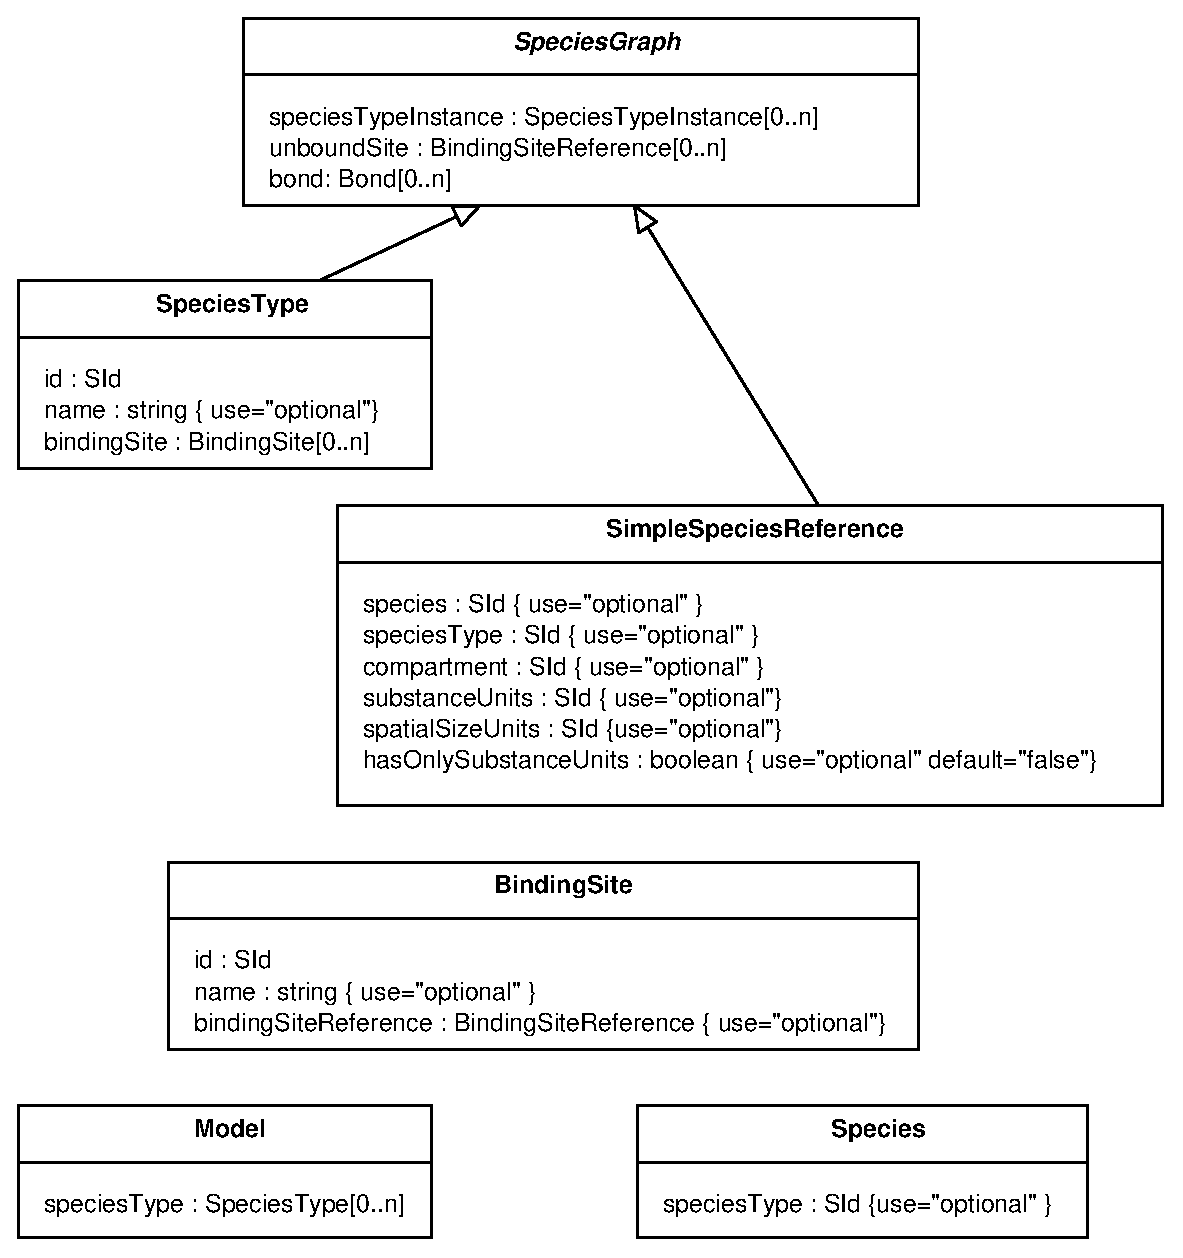
\includegraphics[scale = 0.7]{multi-component-species-uml.eps}
  \caption{The types and attributes introduced into SBML by this proposal, part 1.  This diagram
  only shows new classes and fields: all SBML Level 2 structures are assumed to be present.}
  \label{fig:multi-component-species-uml}
\end{figure}
\begin{figure}[h]
  \vspace*{8pt}
  \centering
  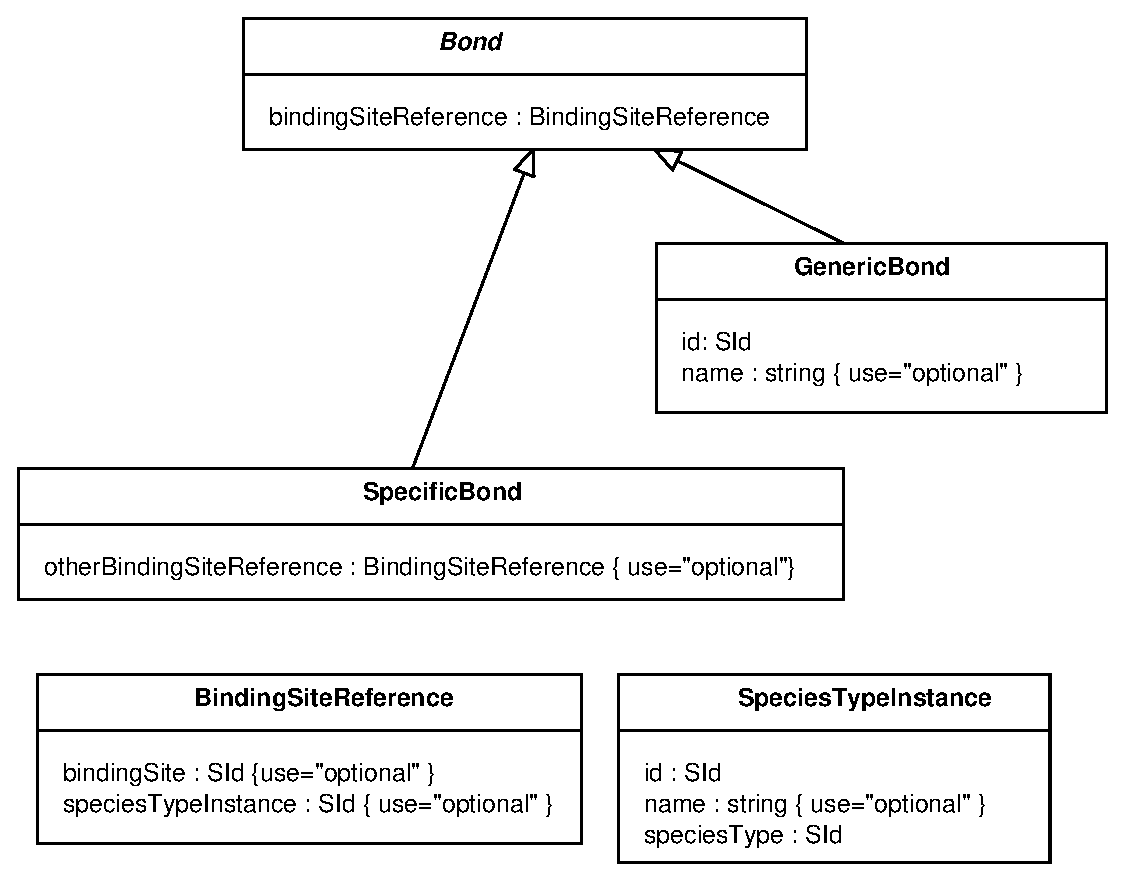
\includegraphics[scale = 0.7]{multi-component-species-uml2.eps}
  \caption{The types and attributes introduced into SBML by this proposal, part 2.  This diagram
  only shows new classes and fields: all SBML Level 2 structures are assumed to be present.}
  \label{fig:multi-component-species-uml2}
\end{figure}

The proposal is described more formally in section~\ref{sec:definitions}.
Section~\ref{sec:definitions} can be considered as a reference section.
The Appendix includes tables which summarize the new XML components that
are introduced by this proposal to the XML encoding of SBML.

\clearpage

\section{Tutorial on the Proposed Features}
\label{sec:tutorial}
\subsection{The Definition of Chemical Entities across Compartments}
\label{sec:commonspecies}

Consider a model where we have a chemical entity which exists in more than one compartment.
for example we might wish to model Aspartate in a Cytosol compartment and in the Mitochondrial Matrix.
In SBML Level 2 we have represent each pool of Aspartate located in a separate compartment, using a
\class{Species} structure as shown in Figure~\ref{fig:malate_aspartate_shuttle1-xml}

\begin{figure}[h]
\begin{example}
<model id="malate_aspartate_shuttle1">
    <listOfCompartments>
        <compartment id="Cytosol"/>
        <compartment id="Mitochondrial_Matrix"/>
    </listOfCompartments>
    <listOfSpecies>
        <species id="Aspartate_in_Cytosol" compartment="Cytosol"/>
        <species id="Aspartate_in_Mitochondrial_Matrix" compartment="Mitochondrial_Matrix"/>
    </listOfSpecies>
</model>
\end{example}
\caption{\texttt{malate\_aspartate\_shuttle1} Model with the same type of chemical entity located in
different compartments.} 
\label{fig:malate_aspartate_shuttle1-xml}
\end{figure}

In SBML Level 2 there is no formal way to relate these species together.  Under this proposal
we do this by representing the Aspartate with a \class{SpeciesType} structure and then
referring to the \class{SpeciesType} from the \class{Species} structures.  We can thus transform the 
\texttt{malate\_aspartate\_shuttle1} Model in Figure~\ref{fig:malate_aspartate_shuttle1-xml} to that
shown in Figure~\ref{fig:malate_aspartate_shuttle2-xml}.

\begin{figure}[h]
\begin{example}
<model id="malate_aspartate_shuttle2">
    <listOfCompartments>
        <compartment id="Cytosol"/>
        <compartment id="Mitochondrial_Matrix"/>
    </listOfCompartments>
    <listOfSpeciesTypes>
        <speciesType id="Aspartate"/>
    </listOfSpeciesTypes>
    <listOfSpecies>
        <species
            id="Aspartate_in_Cytosol"
            speciesType="Aspartate"
            compartment="Cytosol"/>
        <species
            id="Aspartate_in_Mitochondrial_Matrix"
            speciesType="Aspartate"
            compartment="Mitochondrial_Matrix"/>
    </listOfSpecies>
</model>
\end{example}
\caption{\texttt{malate\_aspartate\_shuttle2} Model which uses a \class{SpeciesType} to link species of
the same type of chemical entity that are located in different compartments.} 
\label{fig:malate_aspartate_shuttle2-xml}
\end{figure}

This model does not introduce any new variables that are not present in
\texttt{malate\_aspartate\_shuttle1} it simply identifies \texttt{Aspartate\_in\_Cytosol}
and \texttt{Aspartate\_in\_Mitochondrial\_Matrix} as being separate pools of the same chemical entity.
You cannot refer to \class{SpeciesType} structures from MathML structures under this proposal.

The \texttt{malate\_aspartate\_shuttle1} example is still a valid model under this proposal.
For backwards compatibility the \attrib{speciesType} attribute on \class{Species} is not
mandatory.

It is not possible to locate a \class{SpeciesType} in a \class{Compartment} more than once
i.e. it is not possible for two \class{Species} structures to have the same
\attrib{speciesType} and \attrib{compartment} values.

\subsection{Generalized Reactions: The Definition of Reactions across Compartments}
\label{sec:commonreaction}

Just as we would wish to give a common identify to chemical entities distributed across several
compartments we would wish to have some common object describing reactions between those chemical
entities that is independent of the compartments in which the reactions occur.

For example consider the representation of the transamination reaction, a reversible reaction
that converts Aspartate to Oxaloacetate in both the Cytosol and Mitochondrial Matrix.

We could extend \texttt{malate\_aspartate\_shuttle2} using the SBML Level 2 form as shown in
Figure~\ref{fig:malate_aspartate_shuttle3-xml}

\begin{figure}[h]
\begin{example}
<model id="malate_aspartate_shuttle3">
    <listOfCompartments>
        <compartment id="Cytosol"/>
        <compartment id="Mitochondrial_Matrix"/>
    </listOfCompartments>
    <listOfSpeciesTypes>
        <speciesType id="Aspartate"/>
        <speciesType id="Oxaloacetate"/>
    </listOfSpeciesTypes>
    <listOfSpecies>
        <species
            id="Aspartate_in_Cytosol"
            speciesType="Aspartate"
            compartment="Cytosol"/>
        <species
            id="Aspartate_in_Mitochondrial_Matrix"
            speciesType="Aspartate"
            compartment="Mitochondrial_Matrix"/>
        <species
            id="Oxaloacetate_in_Cytosol"
            speciesType="Oxaloacetate"
            compartment="Cytosol"/>
        <species
            id="Oxaloacetate_in_Mitochondrial_Matrix"
            speciesType="Oxaloacetate"
            compartment="Mitochondrial_Matrix"/>
    </listOfSpecies>
    <listOfReactions>
        <reaction id="Transamination_in_Cytosol" reversible="true">
            <listOfReactants>
                <speciesReference species="Aspartate_in_Cytosol"/>
            </listOfReactants>
            <listOfProducts>
                <speciesReference species="Oxaloacetate_in_Cytosol"/>
            </listOfProducts>
        </reaction>
        <reaction id="Transamination_in_Mitochondrial_Matrix" reversible="true">
            <listOfReactants>
                <speciesReference species="Aspartate_in_Mitochondrial_Matrix"/>
            </listOfReactants>
            <listOfProducts>
                <speciesReference species="Oxaloacetate_in_Mitochondrial_Matrix"/>
            </listOfProducts>
        </reaction>
    </listOfReactions>
</model>
\end{example}
\caption{The \texttt{malate\_aspartate\_shuttle3} model which has duplicate reactions for each
compartment.} 
\label{fig:malate_aspartate_shuttle3-xml}
\end{figure}

Under this proposal we can replace the 2 reactions in Figure~\ref{fig:malate_aspartate_shuttle3-xml} 
with a single reaction structure as shown in Figure~\ref{fig:malate_aspartate_shuttle4-xml}

\begin{figure}[h]
\begin{example}
<model id="malate_aspartate_shuttle4">
    <listOfCompartments>
        <compartment id="Cytosol"/>
        <compartment id="Mitochondrial_Matrix"/>
    </listOfCompartments>
    <listOfSpeciesTypes>
        <speciesType id="Aspartate"/>
        <speciesType id="Oxaloacetate"/>
    </listOfSpeciesTypes>
    <listOfSpecies>
        <species
            id="Aspartate_in_Cytosol"
            speciesType="Aspartate"
            compartment="Cytosol"/>
        <species
            id="Aspartate_in_Mitochondrial_Matrix"
            speciesType="Aspartate"
            compartment="Mitochondrial_Matrix"/>
        <species
            id="Oxaloacetate_in_Cytosol"
            speciesType="Oxaloacetate"
            compartment="Cytosol"/>
        <species
            id="Oxaloacetate_in_Mitochondrial_Matrix"
            speciesType="Oxaloacetate"
            compartment="Mitochondrial_Matrix"/>
    </listOfSpecies>
    <listOfReactions>
        <reaction id="Transamination" reversible="true">
            <listOfReactants>
                <speciesReference speciesType="Aspartate"/>
            </listOfReactants>
            <listOfProducts>
                <speciesReference speciesType="Oxaloacetate"/>
            </listOfProducts>
        </reaction>
    </listOfReactions>
</model>
\end{example}
\caption{The \texttt{malate\_aspartate\_shuttle4} model which has a single reaction which is potentially
located in all compartments.} 
\label{fig:malate_aspartate_shuttle4-xml}
\end{figure}

The reaction structure represents the set of reactions which occurs in all compartments where 
the reactant or product are located.  This reaction would only occur where the reactant is located
if the reaction was not reversible.  All the \class{SimpleSpeciesReference} structures refer to 
species in the same compartment.  This means that, under this proposal, it is not possible to define
a transport reaction, that is a reaction which moves chemical entities between compartments,
using this simple form.  However a variant form is described in
section~\ref{sec:locatedspeciesreferences} which employs a similar form to transport reactions.

\subsubsection{Defining the explicit location of a \class{SimpleSpeciesReference}}
\label{sec:locatedspeciesreferences}

The location of a species pool can be made explicit in a \class{SimpleSpeciesReference} structure
without referring to a \class{Species} structure.  This can be achieved by using the proposed optional
\attrib{compartment} field which refers to a \class{Compartment} structure to indicate the 
location of the given \class{SpeciesType}.

For example consider the transport reaction shown in Figure~\ref{fig:Malate_Transport-xml}
which can be added to the model in Figure~\ref{fig:malate_aspartate_shuttle4-xml}.

\begin{figure}[h]
\begin{example}
<reaction id="Malate_Transport" reversible="false">
    <listOfReactants>
        <speciesReference speciesType="Malate" compartment="Cytosol"/>
    </listOfReactants>
    <listOfProducts>
        <speciesReference speciesType="Malate" compartment="Mitochondrial_Matrix"/>
    </listOfProducts>
</reaction>
\end{example}
\caption{The \texttt{Malate\_Transport} model a transport reaction which refers to \class{SpeciesType}
structures in specific compartments.} 
\label{fig:Malate_Transport-xml}
\end{figure}


\emph{This feature could be introduced later in the SBML development road map.
It is however an essential component of features introduced later.}

All the \class{SimpleSpeciesReference} structures of a reaction should simultaneously either
(a) be located (i.e. have values for the \attrib{species} or \attrib{compartment} attributes);
or (b) apply to any compartment (i.e. not have values for the \attrib{species} and \attrib{compartment}
attributes). \emph{This restriction is not essential but simplifies the interpretation of
the proposed format}.

\subsubsection{Defining Kinetic Laws for Generalized Reactions}

As defined in the examples above it is not possible to compose the kinetic law of these generalized
reactions since there is no symbol that refers to either the modifiers, reactants or products or the
reaction species pools.  However under this proposal the \attrib{id} field of a
\class{SimpleSpeciesReference} becomes a symbol that can be used in the \class{KineticLaw} of the 
enclosing \class{Reaction}.

\emph{Here I am assuming that the \attrib{id} field on \class{SimpleSpeciesReference} is introduced by a
new version of SBML Level 2 as proposed by ??? in ???. This \attrib{id} field is in the global symbol
namespace despite, for the purposes of this proposal, only having scope in the enclosing
\class{Reaction}.  If this is problematic then perhaps we could consider an additional attribute to
declare the symbol.}

As example Figure~\ref{fig:Transamination-xml} shows the \texttt{Transamination} reaction, from model
\texttt{malate\_aspartate\_shuttle4}, modified to include a rate law.

\begin{figure}[h]
\begin{example}
<reaction id="Transamination" reversible="true">
    <listOfReactants>
        <speciesReference id="S1" speciesType="Aspartate"/>
    </listOfReactants>
    <listOfProducts>
        <speciesReference speciesType="Oxaloacetate"/>
    </listOfProducts>
    <kineticLaw>
        <math xmlns="http://www.w3.org/1998/MathMathML">
            <apply>
                <times/>
                <cn>1.1</cn>
                <ci>S1</ci>
            </apply> 
        </math>
    </kineticLaw>
</reaction>
\end{example}
\caption{The \texttt{Transamination} reaction from
Figure~\ref{fig:malate_aspartate_shuttle4-xml} modified to include a kinetic law.} 
\label{fig:Transamination-xml}
\end{figure}

\subsubsection{The Unit Attributes of \class{SimpleSpeciesReference}}

To make the units of species explicit in kinetic laws under this proposal 
\class{SimpleSpeciesReference} structures have the attributes \attrib{substanceUnits},
\attrib{spatialSizeUnits} and \attrib{hasOnlySubstanceUnits}.  These have the same semantics as
the corresponding attributes on \class{Species}.  
When a \class{SimpleSpeciesReference} structure matches with a \class{Species} structure
the unit attributes of the \class{SimpleSpeciesReference} structure should default to the
\class{Species} attributes and/or be exactly equivalent to them.  

EXAMPLE HERE

\subsection{Inferring Species}

Under this proposal \class{Species} structures are used to indicate the initial conditions
and/or attributes of specific pools of chemical entities (species) and don't represent the complete
set of pools.  In SBML Level 2 the model's \attrib{species} list is a complete enumeration of the
pools of chemical entities.  Instead, in this proposal, the set of \class{Species} structures
which have an undefined or non-zero initial amount or concentration, \emph{initial species}, are used 
as a starting point to infer the complete set of species in the model.  The complete set of species
located in a given compartment can be inferred by traversing the reaction
network, defined by the set of \class{Reaction} structures, from the initial species that are located
in the compartment.

So if we consider the model \texttt{malate\_aspartate\_shuttle4} the existence of
\texttt{Oxaloacetate} in the compartment \texttt{Cytosol} can be inferred given the reaction
\texttt{Transamination} and the species \texttt{Aspartate\_in\_Cytosol}.  This means we can omit
the species \texttt{Oxaloacetate\_in\_Cytosol} from the \texttt{malate\_aspartate\_shuttle4} as shown
in Figure~\ref{fig:malate_aspartate_shuttle5-xml}.

\begin{figure}[h]
\begin{example}
<model id="malate_aspartate_shuttle5">
    <listOfCompartments>
        <compartment id="Cytosol"/>
        <compartment id="Mitochondrial_Matrix"/>
    </listOfCompartments>
    <listOfSpeciesTypes>
        <speciesType id="Aspartate"/>
        <speciesType id="Oxaloacetate"/>
    </listOfSpeciesTypes>
    <listOfSpecies>
        <species
            id="Aspartate_in_Cytosol"
            speciesType="Aspartate"
            compartment="Cytosol"/>
        <species
            id="Aspartate_in_Mitochondrial_Matrix"
            speciesType="Aspartate"
            compartment="Mitochondrial_Matrix"/>
    </listOfSpecies>
    <listOfReactions>
        <reaction id="Transamination" reversible="true">
            <listOfReactants>
                <speciesReference speciesType="Aspartate"/>
            </listOfReactants>
            <listOfProducts>
                <speciesReference speciesType="Oxaloacetate"/>
            </listOfProducts>
        </reaction>
    </listOfReactions>
</model>
\end{example}
\caption{The \texttt{malate\_aspartate\_shuttle5} model with a reduced set of initial \texttt{Species}
structures.} 
\label{fig:malate_aspartate_shuttle5-xml}
\end{figure}


\emph{The inference of species could be introduced later in the SBML development road map.
It is however an essential component of features introduced later.}

Just as it is not possible to locate a \class{SpeciesType} in \class{Compartment} more than
once the process of inferring the complete set of species may start from the initial species
set and match with other \class{Species} that have for example a initial concentration of zero.
The inference process does not create duplicate species.

Inferred species, which don't match any \class{Species} structures, always have an initial
concentration or substance amount of zero and are never
constant nor boundary conditions.  This means that constant or boundary condition pools or pools
with any initial concentration must be made explicit using a \class{Species} structure.
Two 
\class{SimpleSpecisReference} structures that refer to the same inferred species should have
the same units.

\emph{The above definition implies that the units of \class{SimpleSpeciesReference} can vary
depending on the inferred species that is being matched with.  It is open question whether this
condition is actually a problem or not}

Reactions of the form used in the example reaction \texttt{Malate\_Transport} fit in with the
inference scheme.  If \texttt{Malate} exists in the
Cytosol then we can infer the existence of a pool of \texttt{Malate} in the
Mitochondrial Matrix.  Given this form of reaction \class{Species} structures are only
required to define the initial conditions of a model.

\subsection{Simple Multi-Component Chemical Entities}
\label{sec:multicomponentspecies}

In this proposal \class{SpeciesType} structures can be composed from instances of other chemical
entities.  For example see model, shown with XML and diagramtic form in
Figure~\ref{fig:pheromone_response}.

\begin{figure}[h]
\begin{example}
<model "Pheromone_response">
    <listOfSpeciesTypes>
        <speciesType id="Ste5"/>
        <speciesType id="Ste11"/>
        <speciesType id="Ste7"/>
        <speciesType id="Fus3"/>
        <speciesType id="SteComplex">
            <listOfSpeciesTypeInstances>
                <speciesTypeInstance id="iSte5" speciesType="Ste5"/>
                <speciesTypeInstance id="iSte11" speciesType="Ste11"/>
                <speciesTypeInstance id="iSte7" speciesType="Ste7"/>
                <speciesTypeInstance id="iFus3" speciesType="Fus3"/>
            </listOfSpeciesTypeInstances>
        </speciesType>
    </listOfSpeciesTypes>
</model>
\end{example}
  \vspace*{8pt}
  \centering
  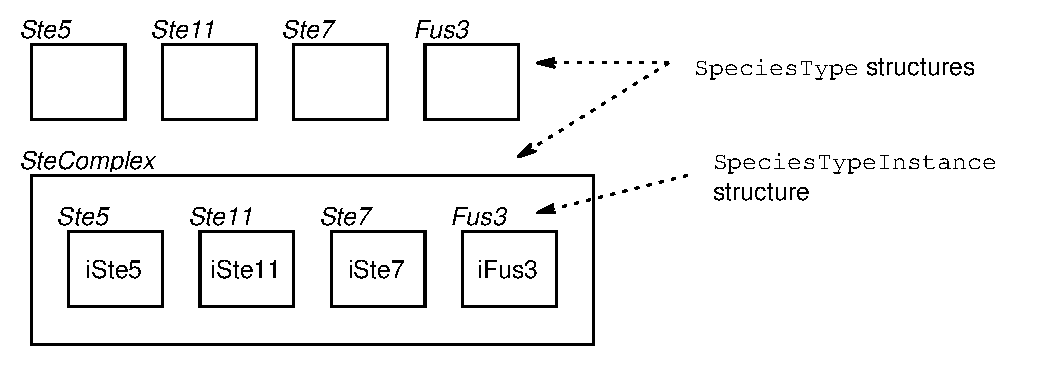
\includegraphics[scale = 0.7]{pheromone_response.eps}
  \caption{The \texttt{Pheromone\_response} model}
  \label{fig:pheromone_response}
\end{figure}

This indicates that \texttt{SteComplex}
is a complex made up of one instance each of the proteins \texttt{Ste5}, \texttt{Ste11}, \texttt{Ste7}
and \texttt{Fus3}.

We can also describe reactions in using this form on \class{SpeciesReference} structures.  For example
we can describe the binding of \texttt{Ste11} to \texttt{Ste5} with the \class{Reaction}
structure shown in Figure~\ref{fig:binding_Ste5_Ste11}.

\begin{figure}[h]
\begin{example}
<reaction id="binding_Ste5_Ste11">
    <listOfReactants>
        <speciesReference speciesType="Ste11"/>
        <speciesReference speciesType="Ste5"/>
    </listOfReactants>
    <listOfProducts>
        <speciesReference>
            <listOfSpeciesTypeInstances>
                <speciesTypeInstance id="iSte5" speciesType="Ste5"/>
                <speciesTypeInstance id="iSte11" speciesType="Ste11"/>
            </listOfSpeciesTypeInstances>
        </speciesReference>
    </listOfProducts>
</reaction>
\end{example}
  \vspace*{8pt}
  \centering
  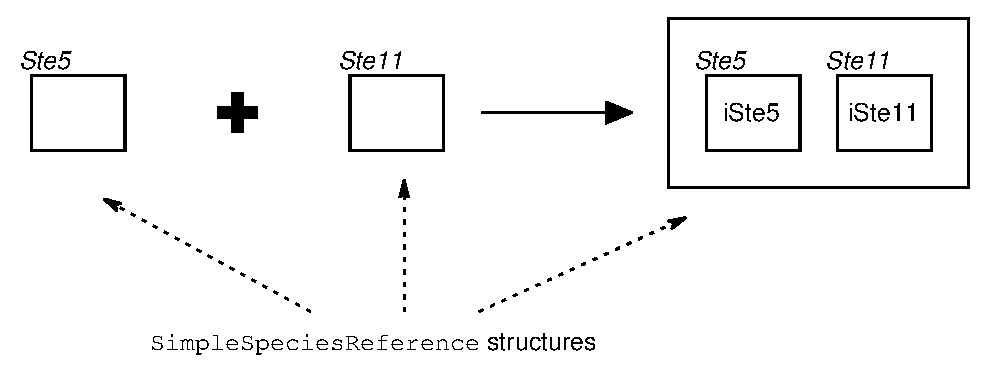
\includegraphics[scale = 0.7]{binding_Ste5_Ste11.eps}
  \caption{The \texttt{binding\_Ste5\_Ste11} reaction, operating in the context of the species types
  defined in Figure~\ref{fig:pheromone_response}}
  \label{fig:binding_Ste5_Ste11}
\end{figure}

Although the the identity of \class{SpeciesTypeInstance} structures is declared in each
\class{SimpleSpeciesReference} structure these identities have scope throughout a reaction.
The \class{SpeciesTypeInstance} \attrib{id} fields with the same value in the same reaction refer
to the same chemical entity.  By giving \class{SpeciesTypeInstance} \attrib{id} fields the same values
in the reactants and products of a reaction we indicate that the entity is only modified by the reaction
rather than being created or destroyed by the reaction.  For example the reaction
\texttt{binding\_Ste5\_Ste11} could be encoded as shown in Figure~\ref{fig:binding_Ste5_Ste11_v2}.

\begin{figure}[h]
\begin{example}
<reaction id="binding_Ste5_Ste11_v2">
    <listOfReactants>
        <speciesReference>
            <listOfSpeciesTypeInstances>
                <speciesTypeInstance id="iSte5" speciesType="Ste5"/>
            </listOfSpeciesTypeInstances>
        </speciesReference>
        <speciesReference>
            <listOfSpeciesTypeInstances>
                <speciesTypeInstance id="iSte11" speciesType="Ste11"/>
            </listOfSpeciesTypeInstances>
        </speciesReference>
    </listOfReactants>
    <listOfProducts>
        <speciesReference>
            <listOfSpeciesTypeInstances>
                <speciesTypeInstance id="iSte5" speciesType="Ste5"/>
                <speciesTypeInstance id="iSte11" speciesType="Ste11"/>
            </listOfSpeciesTypeInstances>
        </speciesReference>
    </listOfProducts>
</reaction>
\end{example}
  \vspace*{8pt}
  \centering
  \includegraphics[scale = 0.7]{binding_Ste5_Ste11_v2.eps}
  \caption{The \texttt{binding\_Ste5\_Ste11\_v2} reaction}
  \label{fig:binding_Ste5_Ste11_v2}
\end{figure}

This encoding indicates that, for the purposes of the model, \texttt{Ste5} and \texttt{Ste11}
are not modified when they bond.  The distinction between \texttt{binding\_Ste5\_Ste11}
and \texttt{binding\_Ste5\_Ste11\_v2} is only descriptive however the latter form
is used as the basis for more complex semantics later. 

A model like \texttt{pheromone\_response} with or without characterized reaction including kinetic laws
doesn't encapsulate a model that can be simulated because it does not specify the initial concentration
or location of pools of the defined chemical entities.

\subsection{Multi-component Chemical Entities with explicit bonds}
\label{sec:explicitbonds}

The forms described in section~\ref{sec:multicomponentspecies} capture some but not all
the relevant knowledge of chemical entities that we might wish to model.  In this section I
describe how chemical bond information is captured.
The bond information on a \class{SimpleSpeciesReference} or a \class{SpeciesType} turns into a
graph linking the \class{SpeciesTypeInstance} structures together.
The description of a structures using chemical
bonds requires the identification of binding sites on \class{SpeciesType} structures and
then the enumeration of the bonds on those binding sites.  We can redefine the model
\texttt{pheromone\_response} along these lines as shown in Figure~\ref{fig:pheromone_response_v2} on
page~\pageref{fig:pheromone_response_v2}.

\begin{figure}[h]
\begin{example}
<model "pheromone_response_v2">
    <listOfSpeciesTypes>
        <speciesType id="Ste5">
            <listOfBindingSites>
                <bindingSite id="r241">
                <bindingSite id="r463">
                <bindingSite id="r744">
            </listOfBindingSites>
        </speciesType>
        <speciesType id="Ste11"/>
            <listOfBindingSites>
                <bindingSite id="site">
            </listOfBindingSites>
        </speciesType>
        <speciesType id="Ste7"/>
            <listOfBindingSites>
                <bindingSite id="site">
            </listOfBindingSites>
        </speciesType>
        <speciesType id="Fus3"/>
            <listOfBindingSites>
                <bindingSite id="site">
            </listOfBindingSites>
        </speciesType>
        <speciesType id="SteComplex">
            <listOfSpeciesTypeInstances>
                <speciesTypeInstance id="iSte5" speciesType="Ste5"/>
                <speciesTypeInstance id="iSte11" speciesType="Ste11"/>
                <speciesTypeInstance id="iSte7" speciesType="Ste7"/>
                <speciesTypeInstance id="iFus3" speciesType="Fus3"/>
            </listOfSpeciesTypeInstances>
            <listOfBonds>
                <specificBond>
                    <bindingSiteReference speciesTypeInstance="iSte5" bindingSite="r241"/>
                    <otherBindingSiteReference
                        speciesTypeInstance="iFus3" bindingSite="site"/>
                </specificBond>
                <specificBond>
                    <bindingSiteReference speciesTypeInstance="iSte5" bindingSite="r463"/>
                    <otherBindingSiteReference
                        speciesTypeInstance="iSte11" bindingSite="site"/>
                </specificBond>
                <specificBond>
                    <bindingSiteReference speciesTypeInstance="iSte5" bindingSite="r744"/>
                    <otherBindingSiteReference
                        speciesTypeInstance="iSte7" bindingSite="site"/>
                </specificBond>
            </listOfBonds>
        </speciesType>
    </listOfSpeciesTypes>
</model>
\end{example}
  \vspace*{8pt}
  \centering
  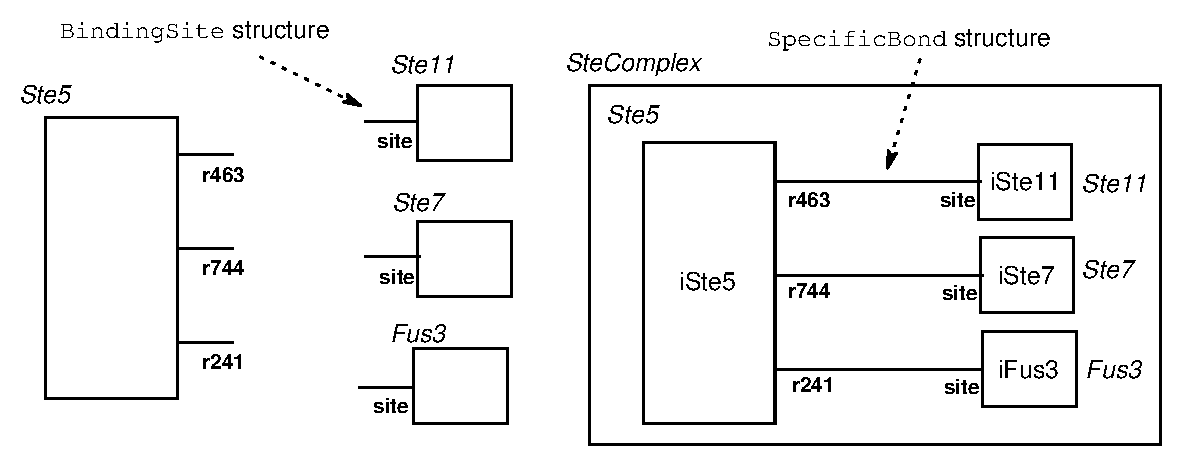
\includegraphics[scale = 0.7]{pheromone_response_v2.eps}
  \caption{The
  \texttt{pheromone\_response\_v2}
  model.}
  \label{fig:pheromone_response_v2}
\end{figure}

The \class{SpecificBond} structures used in the \texttt{pheromone\_response\_v2} model can also be
used to indicate unbound binding sites as shown the reaction in Figure~\ref{fig:binding_Ste5_Ste11_v3} on
page~\pageref{fig:binding_Ste5_Ste11_v3}.

\begin{figure}[h]
\begin{example}
<reaction id="binding_Ste5_Ste11_v3">
    <listOfReactants>
        <speciesReference>
            <listOfSpeciesTypeInstances>
                <speciesTypeInstance id="iSte5" speciesType="Ste5"/>
            </listOfSpeciesTypeInstances>
            <listOfBonds>
                <specificBond>
                    <bindingSiteReference speciesTypeInstance="iSte5" bindingSite="r241"/>
                </specificBond>
                <specificBond>
                    <bindingSiteReference speciesTypeInstance="iSte5" bindingSite="r463"/>
                </specificBond>
                <specificBond>
                    <bindingSiteReference speciesTypeInstance="iSte5" bindingSite="r744"/>
                </specificBond>
            </listOfBonds>
        </speciesReference>
        <speciesReference>
            <listOfSpeciesTypeInstances>
                <speciesTypeInstance id="iSte11" speciesType="Ste11"/>
            </listOfSpeciesTypeInstances>
            <listOfBonds>
                <specificBond>
                    <bindingSiteReference speciesTypeInstance="iSte11" bindingSite="site"/>
                </specificBond>
            </listOfBonds>
         </speciesReference>
    </listOfReactants>
    <listOfProducts>
        <speciesReference>
            <listOfSpeciesTypeInstances>
                <speciesTypeInstance id="iSte5" speciesType="Ste5"/>
                <speciesTypeInstance id="iSte11" speciesType="Ste11"/>
            </listOfSpeciesTypeInstances>
            <listOfBonds>
                <specificBond>
                    <bindingSiteReference speciesTypeInstance="iSte5" bindingSite="r241"/>
                </specificBond>
                <specificBond>
                    <bindingSiteReference speciesTypeInstance="iSte5" bindingSite="r463"/>
                    <otherBindingSiteReference
                        speciesTypeInstance="iSte11" bindingSite="site"/>
                </specificBond>
                <specificBond>
                    <bindingSiteReference speciesTypeInstance="iSte5" bindingSite="r744"/>
                </specificBond>
            </listOfBonds>
        </speciesReference>
    </listOfProducts>
</reaction>
\end{example}
  \vspace*{8pt}
  \centering
  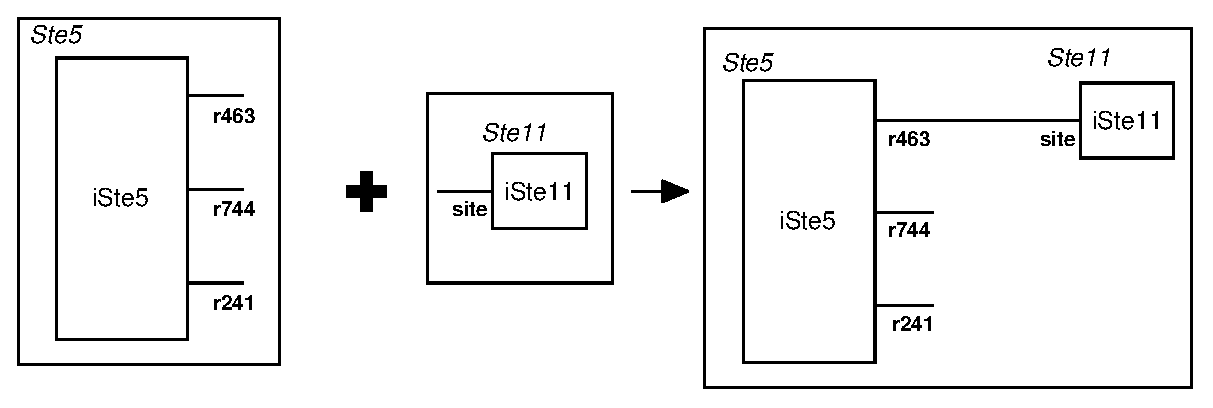
\includegraphics[scale = 0.7]{binding_Ste5_Ste11_v3.eps}
  \caption{The \texttt{binding\_Ste5\_Ste11\_v3} reaction}
  \label{fig:binding_Ste5_Ste11_v3}
\end{figure}

A \class{SpeciesType} structure must not leave the state of a binding site undefined or ambiguous.
Section~\ref{sec:generalizedreactions} describes how a \class{SimpleSpeciesReference} can refer to 
several different \class{SpeciesType} structures where the class represents a range of states for one
or more binding sites.

The level of decomposition of a biochemical system into chemical entities and their binding sites and
bonds is not defined by this proposal.  This proposal is designed to support arbitrary decomposition
schemes which capture knowledge at different resolutions in the same model. The
underlying chemistry represented by a given binding site state is also not defined by this proposal.

An underlying principle of this proposal is that the binding representation described in this section
can be used to represent the reversible covalent modification of proteins including, for example,
phosphorylation and dephosphorylation.  The example model shown in
Figure~\ref{fig:Phosphorylation_model-xml} on page~\pageref{fig:Phosphorylation_model-xml}represents
the phosphorylation of \texttt{Ste11} by \texttt{Ste20}.  A diagram of this model is shown in
Figure~\ref{fig:Phosphorylation_model} on page~\pageref{fig:Phosphorylation_model}.

\begin{figure}[h]
\begin{example}
<model id="Phosphorylation_model">
    <listOfSpeciesTypes>
        <speciesType id="Phosphate">
            <listOfBindingSites>
                <bindingSite id="site"/>
            </listOfBindingSites>
        </speciesType>
        <speciesType id="Ste20"/>
        <speciesType id="Ste11">
            <listOfBindingSites>
                <bindingSite id="S302"/>
                <bindingSite id="T307"/>
            </listOfBindingSites>
        </speciesType>
    </listofSpeciesTypes>
    <listOfReactions>
        <reaction id="Phosphorylation">
            <listOfReactants>
                <speciesReference>
                    <listOfSpeciesTypeInstances>
                        <speciesTypeInstance id="iSte11" speciesType="Ste11"/>
                    </listOfSpeciesTypeInstances>
                    <listOfBonds>
                        <specificBond>
                            <bindingSiteReference
                                speciesTypeInstance="iSte11" bindingSite="S302"/>
                        </specificBond>
                        <specificBond>
                            <bindingSiteReference
                                speciesTypeInstance="iSte11" bindingSite="T307"/>
                        </specificBond>
                    </listOfBonds>
                </speciesReference>
            </listOfReactants>
            <listOfProducts>
                <speciesReference>
                    <listOfSpeciesTypeInstances>
                        <speciesTypeInstance id="iSte11" speciesType="Ste11"/>
                        <speciesTypeInstance id="iPhosphate_1" speciesType="Phosphate"/>
                        <speciesTypeInstance id="iPhosphate_2" speciesType="Phosphate"/>
                    </listOfSpeciesTypeInstances>
                    <listOfBonds>
                        <specificBond>
                            <bindingSiteReference speciesTypeInstance="iSte11"
                                bindingSite="S302"/>
                            <otherBindingSiteReference
                                speciesTypeInstance="iPhosphate_1" bindingSite="site"/>
                        </specificBond>
                        <specificBond>
                            <bindingSiteReference
                                speciesTypeInstance="iSte11" bindingSite="T307"/>
                            <otherBindingSiteReference
                                speciesTypeInstance="iPhosphate_2" bindingSite="site"/>
                        </specificBond>
                    </listOfBonds>
                </speciesReference>
            </listOfProducts>
            <listOfModifiers>
                <modifierSpeciesReference>
                    <listOfSpeciesTypeInstances>
                        <speciesTypeInstance id="iSte20" speciesType="Ste20"/>
                    </listOfSpeciesTypeInstances>
                </modifierSpeciesReference>
            </listOfModifiers>
        </reaction>
    </listOfReactions>
<model>
\end{example}
  \caption{The \texttt{Phosphorylation\_model} model, a diagram of this model is shown in
  Figure~\ref{fig:Phosphorylation_model}.}
  \label{fig:Phosphorylation_model-xml}
\end{figure}

\begin{figure}[h]
  \vspace*{8pt}
  \centering
  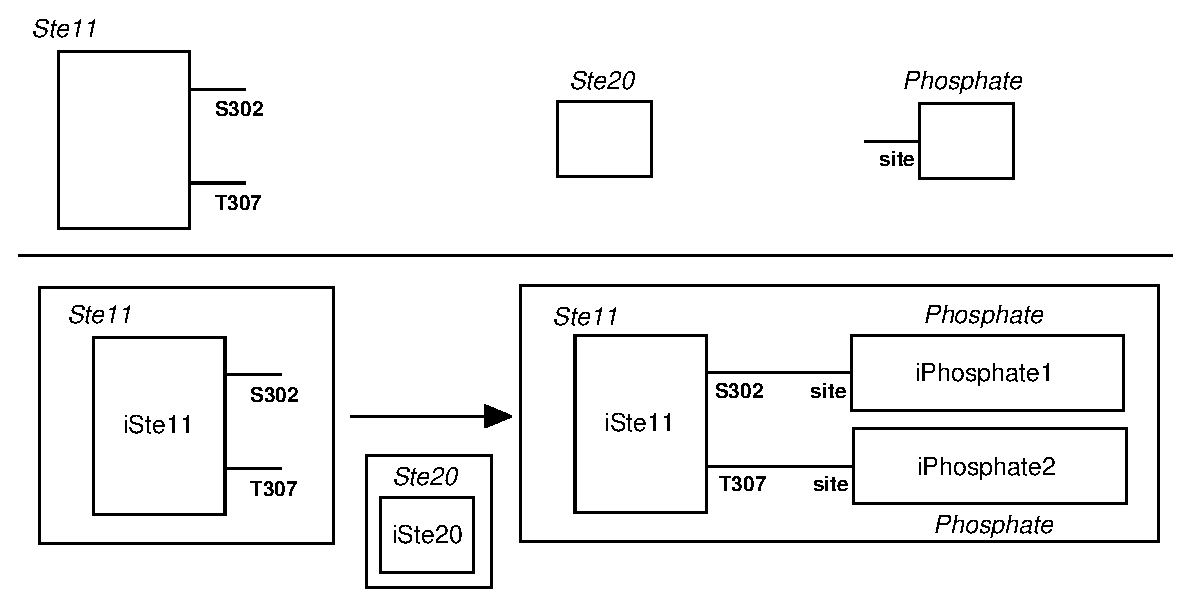
\includegraphics[scale = 0.7]{Phosphorylation-model.eps}
  \caption{Diagram of the \texttt{Phosphorylation\_model} model}
  \label{fig:Phosphorylation_model}
\end{figure}

This model deliberately does not model the involvement of ATP or ADP molecules demonstrating
how the level of detail of the biological knowledge captured by the proposed standard is arbitrary.
As a result not all the instances of species types in the list of reactants are present in the
list of products.  This is valid in this proposal: the structural details of chemical entity
transformation do not have to be fully elucidated.  In fact the reaction shown in
Figure~\ref{fig:demo} on page~\pageref{fig:demo} is valid even if it is implausible from a biochemical
perspective.

\begin{figure}[h]

\begin{example}
<model id="demo">
    <listOfSpeciesTypes>
        <speciesType id="Ste20"/>
        <speciesType id="Ste11"/>
    </listofSpeciesTypes>
    <listOfReactions>
        <reaction id="Implausible">
            <listOfReactants>
                <speciesReference>
                    <listOfSpeciesTypeInstances>
                        <speciesTypeInstance id="iSte11" speciesType="Ste11"/>
                    </listOfSpeciesTypeInstances>
                </speciesReference>
            </listOfReactants>
            <listOfProducts>
                <speciesReference>
                    <listOfSpeciesTypeInstances>
                        <speciesTypeInstance id="iSte20" speciesType="Ste20"/>
                    </listOfSpeciesTypeInstances>
                </speciesReference>
            </listOfModifiers>
        </reaction>
    </listOfReactions>
</model>
\end{example}
  \vspace*{8pt}
  \centering
  \includegraphics[scale = 0.7]{demo.eps}
  \caption{The \texttt{demo} model which shows how a reaction operating on
  components can transform those components.}
  \label{fig:demo}
\end{figure}

\class{SpeciesGraph} structures, i.e. \class{SpeciesType} and \class{SimpleSpeciesReference} structures,
can contain a number of disconnected components.  In detail this means that a list of \class{Bond}
structures in a \class{SpeciesGraph} does not have to comprise a connected graph.  As an example the
consider the model shown in Figure~\ref{fig:disconnected_parts-xml} on
page~\pageref{fig:disconnected_parts-xml}.  A diagram of this model is shown in
Figure~\ref{fig:disconnected_parts} on page~\pageref{fig:disconnected_parts}.

\begin{figure}[h]
\begin{example}
<model id="disconnected_parts">
    <listOfSpeciesTypes>
        <speciesType id="A"/>
        <speciesType id="B">
            <listOfBindingSites>
                <bindingSite id="b">
            </listOfBidingSites>
        </speciesType>
        <speciesType id="C">
            <listOfBindingSites>
                <bindingSite id="c">
            </listOfBidingSites>
        </speciesType>
        <speciesType id="D">
            <listOfSpeciesTypeInstances>
                <speciesTypeInstance id="iA" speciesType="A"/>                
                <speciesTypeInstance id="iB" speciesType="B"/>                
                <speciesTypeInstance id="iC" speciesType="C"/>                
            </listOfSpeciesTypeInstances>
            <listOfBonds>
                <specificBond>
                    <bindingSiteReference speciesTypeInstance="iB" bindingSite="b"/>
                    <otherBindingSiteReference speciesTypeInstance="iC" bindingSite="c"/>
                </specificBond>
            </listOfBonds
        </speciesType>
    </listOfSpeciesTypes>
    <listOfReactions>
        <listOfReactants>
            <speciesReference>
                <listOfSpeciesTypeInstances>
                    <speciesTypeInstance id="iA" speciesType="A"/>                
                 </listOfSpeciesTypeInstances>              
            </speciesReference>
            <speciesReference>
                <listOfSpeciesTypeInstances>
                    <speciesTypeInstance id="iB" speciesType="B"/>                
                    <speciesTypeInstance id="iC" speciesType="C"/>                
                </listOfSpeciesTypeInstances>
                <listOfBonds>
                    <specificBond>
                        <bindingSiteReference speciesTypeInstance="iB" bindingSite="b"/>
                        <otherBindingSiteReference speciesTypeInstance="iC" bindingSite="c"/>
                    </specificBond>
                </listOfBonds
            </speciesReference>
        </listOfReactants>
        <listOfProducts>
            <speciesReference>
                <listOfSpeciesTypeInstances>
                    <speciesTypeInstance id="iA" speciesType="A"/>                
                    <speciesTypeInstance id="iB" speciesType="B"/>                
                    <speciesTypeInstance id="iC" speciesType="C"/>                
                </listOfSpeciesTypeInstances>
                <listOfBonds>
                    <specificBond>
                        <bindingSiteReference speciesTypeInstance="iB" bindingSite="b"/>
                        <otherBindingSiteReference speciesTypeInstance="iC" bindingSite="c"/>
                    </specificBond>
                </listOfBonds
            </speciesReference>
        </listOfProducts>
    </listOfReactions>
</model>
\end{example}
  \caption{The \texttt{disconnected\_parts} model which shows how reactions can operate on
  disconnected components.}
  \label{fig:disconnected_parts-xml}
\end{figure}

\begin{figure}[h]
  \vspace*{8pt}
  \centering
  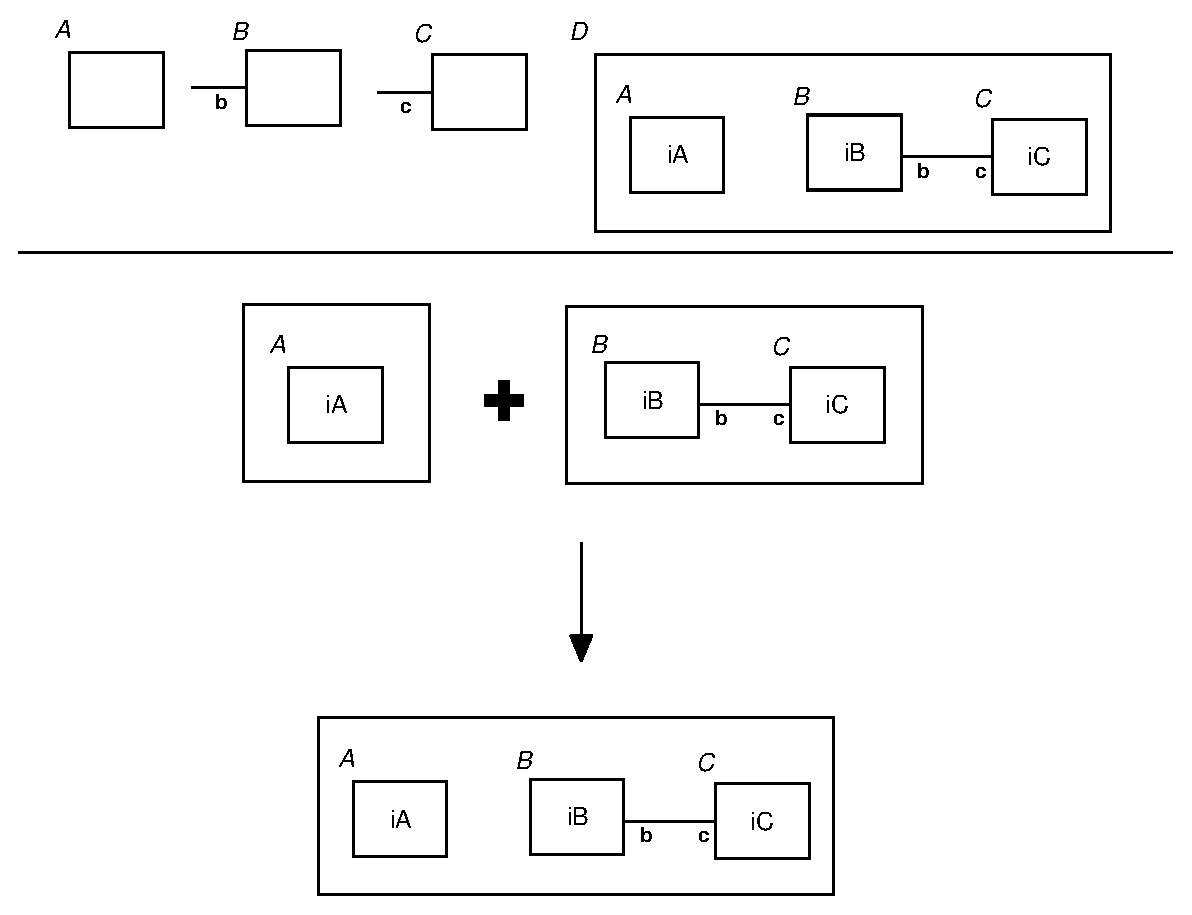
\includegraphics[scale = 0.7]{disconnected_parts.eps}
  \caption{A diagram of the \texttt{disconnected\_parts} model.}
  \label{fig:disconnected_parts}
\end{figure}

\subsection{Reactions generalized to cover classes of Multi-component Chemical Entities}
\label{sec:generalizedreactions}

Under this proposal the bonding concept is extended in reactions so that it is possible 
for a reactant, product or modifier to refer to set of closely related species that have a 
similar but not identical chemical structure.  
This is achieved the use of \class{GenericBond} structures within \class{SimpleSpeciesReference}
structures.
\class{GenericBond} is a alternative \class{Bond} type.  The reactions containing containing a
\class{GenericBond} can potentially
apply to a large set of species thus reducing the number of reactions that need to be enumerated in
a given system.
When a reaction is applied to the given state of one or more reactants, a \class{GenericBond} structure
in the reaction is assigned the state of a binding site to a variable.  The assignment can be to
an empty entity if the match is to an empty binding site or to a unspecified binding site on
an unspecified chemical entity.  This binding site state is transferred from the reactants to the
assigned to a binding site in among the products.

The simple abstract example model shown in Figure~\ref{fig:generalized-xml} on
page~\pageref{fig:generalized-xml} uses this generalization mechanism redundantly.
A diagraom of this model is shown in Figure~\ref{fig:generalized} on
page~\pageref{fig:generalized}.
The reaction \texttt{generic} defines how entities \texttt{A} and \texttt{B} bind together without
changing the state of one of the binding sites on \texttt{A}.

\begin{figure}[h]
\begin{example}
<model "generalized">
    <listOfSpeciesTypes>
        <speciesType id="A">
            <listOfBindingSites>
                <bindingSite id="a"/>
            </listOfBindingSite>
        </speciesType>
        <speciesType id="B">
            <listOfBindingSites>
                <bindingSite id="b1"/>
                <bindingSite id="b2"/>
            </listOfBindingSites>
        </speciesType>
    </listOfSpeciesTypes>
    <listOfReactions>
        <reaction id="generic">
            <listOfReactants>
                <speciesReference>
                    <listOfSpeciesTypeInstances>
                        <speciesTypeInstance id="iA" speciesType="A"/>                
                    </listOfSpeciesTypeInstances>
                    <listOfBonds>
                        <specificBond>
                            <bindingSiteReference speciesTypeInstance="iA" bindingSite="a"/>
                        </specificBond>
                    </listOfBonds
            </speciesReference>
                <speciesReference>
                    <listOfSpeciesTypeInstances>
                        <speciesTypeInstance id="iB" speciesType="B"/>                
                    </listOfSpeciesTypeInstances>
                    <listOfBonds>
                        <specificBond>
                            <bindingSiteReference speciesTypeInstance="iB" bindingSite="b1"/>
                        </specificBond>
                        <genericBond id="X">
                            <bindingSiteReference speciesTypeInstance="iB" bindingSite="b2"/>
                        </genericBond>
                    </listOfBonds
            </speciesReference>
            </listOfReactants>
            <listOfProducts>
                <speciesReference>
                    <listOfSpeciesTypeInstances>
                        <speciesTypeInstance id="iA" speciesType="A"/>                
                        <speciesTypeInstance id="iB" speciesType="B"/>                
                    </listOfSpeciesTypeInstances>
                    <listOfBonds>
                        <specificBond>
                            <bindingSiteReference speciesTypeInstance="iA" bindingSite="a"/>
                            <bindingSiteReference speciesTypeInstance="iB" bindingSite="b1"/>
                        </specificBond>
                        <genericBond id="X">
                            <bindingSiteReference speciesTypeInstance="iB" bindingSite="b2"/>
                        </genericBond>
                    </listOfBonds
            </speciesReference>
            </listOfProducts>
        </reaction>
    </listOfReactions>
</model>
\end{example}
  \caption{The \texttt{generalized} model which shows how a reaction can be applied to a set
  of chemical entities. A diagram of this model is shown in Figure~\ref{fig:generalized}.}
  \label{fig:generalized-xml}
\end{figure}

\begin{figure}[h]
  \vspace*{8pt}
  \centering
  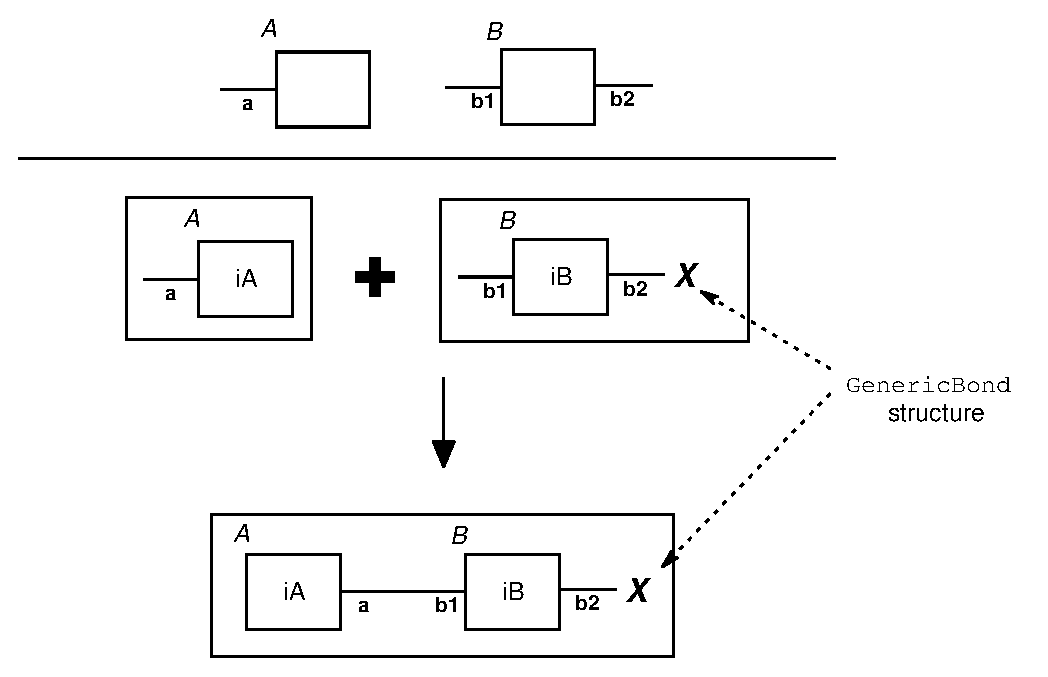
\includegraphics[scale = 0.7]{generalized.eps}
  \caption{A diagram of the \texttt{generalized} model shown in Figure~\ref{fig:generalized-xml}}
  \label{fig:generalized}
\end{figure}

A more concrete example model is shown in fragments in Figures~\ref{fig:non_exclusive_binding_types}
to~\ref{fig:bind_Ste11_Ste5}
on pages~\pageref{fig:non_exclusive_binding_types} to~\pageref{fig:bind_Ste11_Ste5}.
The reactions in Figures~\ref{fig:bind_Ste11_Ste50} and~\ref{fig:bind_Ste11_Ste5}
(which operate on the species types encoded in Figure~\ref{fig:non_exclusive_binding_types})
taken together represent the fact that the binding of
Ste11 to Ste50 is not mutually exclusive to Ste11 binding to Ste5.
Figure~\ref{fig:bind_Ste11_Ste50} shows reaction \texttt{bind\_Ste11\_Ste50} which binds Ste11 to
Ste50 and is generalized to cover all states of the Ste11 to Ste5 binding site.
Figure~\ref{fig:bind_Ste11_Ste5} shows reaction \texttt{bind\_Ste11\_Ste5} binding Ste11 to
Ste5 and is generalized to cover all states of the Ste11 to Ste50 binding site.

\begin{figure}[h]
\begin{example}
<listOfSpeciesTypes>
    <speciesType id="Ste5">
        <listOfBindingSites>
            <bindingSite id="R463_514"/>
        </listOfBindingSites>
    </speciesType>
    <speciesType id="Ste50">
        <listOfBindingSites>
            <bindingSite id="SAM"/>
        </listofBindignSites>
    </speciesType>
    <speciesType id="Ste11">
        <listOfBindingSites>
            <bindingSite id="N_term"/>
            <bindingSite id="SAM"/>
        </listOfBindingSites>
    </speciesType>
</listOfSpeciesTypes>
\end{example}
  \vspace*{8pt}
  \centering
  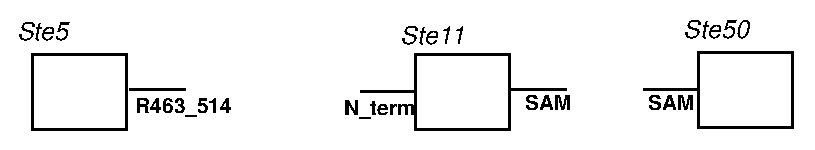
\includegraphics[scale = 0.7]{non_exclusive_binding_types.eps}
  \caption{The species types used in Figures~\ref{fig:bind_Ste11_Ste50}, \ref{fig:bind_Ste11_Ste5}
  and~\ref{fig:bind_Ste11_Ste5_v2}.}
  \label{fig:non_exclusive_binding_types}
\end{figure}

\begin{figure}[h]
\begin{example}
<reaction "bind_Ste11_Ste50">
    <listOfProducts>
        <speciesReference>
            <listOfSpeciesTypeInstances>
                <speciesTypeInstance id="iSte11" speciesType="Ste11"/>
            </listOfSpeciesTypeInstances>
            <listOfBonds>
                <genericBond id="X">
                    <bindingSiteReference bindingSite="N_term" speciesTypeInstance="iSte11"/>
                </genericBond>
                <specificBond>
                    <bindingSiteReference bindingSite="SAM" speciesTypeInstance="iSte11"/>
                </specificBond>
            </listOfBonds>
        </speciesReference>
        <speciesReference>
            <listOfSpeciesTypeInstances>
                <speciesTypeInstance id="iSte50" speciesType="Ste50"/>
            </listOfSpeciesTypeInstances>
            <listOfBonds>
                <specificBond>
                    <bindingSiteReference bindingSite="SAM" speciesTypeInstance="iSte50"/>
                </specificBond>
            </listOfBonds>
        </speciesReference>
    </listOfProducts>
    <listOfReactants>
        <speciesReference>
            <listOfSpeciesTypeInstances>
                <speciesTypeInstance id="iSte11" speciesType="Ste11"/>
                <speciesTypeInstance id="iSte50" speciesType="Ste50"/>
            </listOfSpeciesTypeInstances>
            <listOfBonds>
                <genericBond id="X">
                    <bindingSiteReference bindingSite="N_term" speciesTypeInstance="iSte11"/>
                </genericBond>
                <specificBond>
                    <bindingSiteReference bindingSite="SAM" speciesTypeInstance="iSte11"/>
                    <bindingSiteReference bindingSite="SAM" speciesTypeInstance="iSte50"/>
                </specificBond>
            </listOfBonds>
        </speciesReference>
    </listOfReactants>
</reaction>
\end{example}
  \vspace*{8pt}
  \centering
  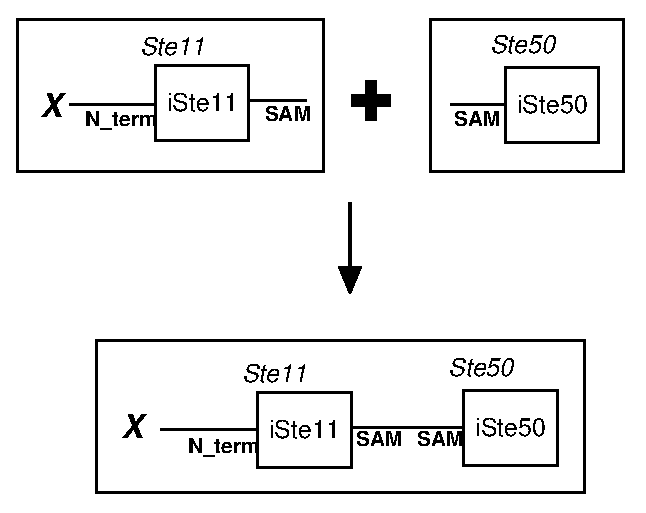
\includegraphics[scale = 0.7]{bind_Ste11_Ste50.eps}
  \caption{The \texttt{bind\_Ste11\_Ste50} binding reaction that operate on the types defined in
  Figure~\ref{fig:non_exclusive_binding_types}}
  \label{fig:bind_Ste11_Ste50}
\end{figure}

\begin{figure}[h]
\begin{example}
<reaction "bind_Ste11_Ste5">
    <listOfProducts>
        <speciesReference>
            <listOfSpeciesTypeInstances>
                <speciesTypeInstance id="iSte11" speciesType="Ste11"/>
            </listOfSpeciesTypeInstances>
            <listOfBonds>
                <genericBond id="X">
                    <bindingSiteReference bindingSite="SAM" speciesTypeInstance="iSte11"/>
                </genericBond>
                <specificBond>
                    <bindingSiteReference bindingSite="N_term" speciesTypeInstance="iSte11"/>
                </specificBond>
            </listOfBonds>
        </speciesReference>
        <speciesReference>
            <listOfSpeciesTypeInstances>
                <speciesTypeInstance id="iSte5" speciesType="Ste5"/>
            </listOfSpeciesTypeInstances>
            <listOfBonds>
                <specificBond>
                    <bindingSiteReference bindingSite="R463_514" speciesTypeInstance="iSte5"/>
                </specificBond>
            </listOfBonds>
        </speciesReference>
    </listOfProducts>
    <listOfReactants>
        <speciesReference>
            <listOfSpeciesTypeInstances>
                <speciesTypeInstance id="iSte11" speciesType="Ste11"/>
                <speciesTypeInstance id="iSte5" speciesType="Ste5"/>
            </listOfSpeciesTypeInstances>
            <listOfBonds>
                <genericBond id="X">
                    <bindingSiteReference bindingSite="SAM" speciesTypeInstance="iSte11"/>
                </genericBond>
                <specificBond>
                    <bindingSiteReference bindingSite="N_term" speciesTypeInstance="iSte11"/>
                    <bindingSiteReference bindingSite="R463_514" speciesTypeInstance="iSte5"/>
                </specificBond>
            </listOfBonds>
        </speciesReference>
    </listOfReactants>
</reaction>
\end{example}
  \vspace*{8pt}
  \centering
  \includegraphics[scale = 0.7]{bind_Ste11_Ste5.eps}
  \caption{The \texttt{bind\_Ste11\_Ste5} reaction that operates on the types defined in
  Figure~\ref{fig:non_exclusive_binding_types}}
  \label{fig:bind_Ste11_Ste5}
\end{figure}

\clearpage
\subsubsection{Missing Binding Sites Infers Unchanged State}

Labelling the connection point of generic bonds enables the modeler a reaction which move an
component of unspecified type from one binding site to another.  However in the majority of cases
the binding site of such a component is not changed by the reaction i.e. the binding site state is
completely irrelevant to the reaction.  The encoding of these cases is simplified:  if a binding site
is both unchanged by a reaction \emph{and} the reaction generalized to cover all states of that
binding site then that binding site is simply omitted from the reaction entirely.  This
is the case for the binding sites referenced by the \class{GenericBond} structures in the
\texttt{bind\_Ste11\_Ste5} reaction shown in Figure~\ref{fig:bind_Ste11_Ste5} on
page~\pageref{fig:bind_Ste11_Ste5} and thus we can
simplify this reaction by omitting the \class{GenericBond} structures as shown in
Figure~\ref{fig:bind_Ste11_Ste5_v2} on page~\pageref{fig:bind_Ste11_Ste5_v2}.

\begin{figure}[h]
\begin{example}
<reaction "bind_Ste11_Ste5">
    <listOfProducts>
        <speciesReference>
            <listOfSpeciesTypeInstances>
                <speciesTypeInstance id="iSte11" speciesType="Ste11"/>
            </listOfSpeciesTypeInstances>
            <listOfBonds>
                <specificBond>
                    <bindingSiteReference bindingSite="N_term" speciesTypeInstance="iSte11"/>
                </specificBond>
            </listOfBonds>
        </speciesReference>
        <speciesReference>
            <listOfSpeciesTypeInstances>
                <speciesTypeInstance id="iSte5" speciesType="Ste5"/>
            </listOfSpeciesTypeInstances>
            <listOfBonds>
                <specificBond>
                    <bindingSiteReference bindingSite="R463_514" speciesTypeInstance="iSte5"/>
                </specificBond>
            </listOfBonds>
        </speciesReference>
    </listOfProducts>
    <listOfReactants>
        <speciesReference>
            <listOfSpeciesTypeInstances>
                <speciesTypeInstance id="iSte11" speciesType="Ste11"/>
                <speciesTypeInstance id="iSte5" speciesType="Ste5"/>
            </listOfSpeciesTypeInstances>
            <listOfBonds>
                <specificBond>
                    <bindingSiteReference bindingSite="N_term" speciesTypeInstance="iSte11"/>
                    <bindingSiteReference bindingSite="R463_514" speciesTypeInstance="iSte5"/>
                </specificBond>
            </listOfBonds>
        </speciesReference>
    </listOfReactants>
</reaction>
\end{example}
  \vspace*{8pt}
  \centering
  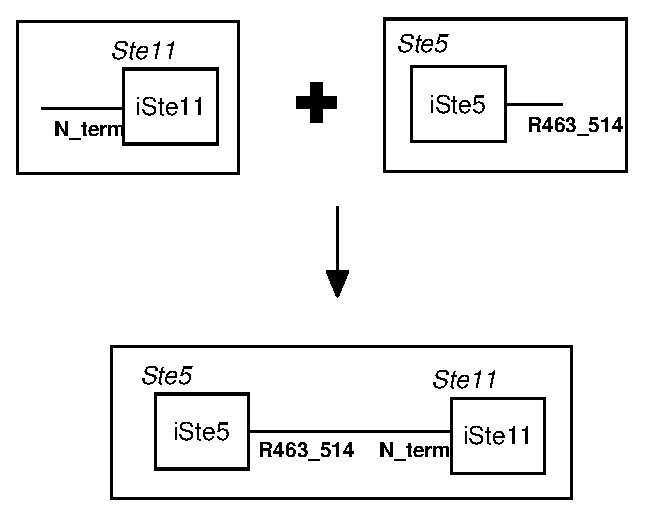
\includegraphics[scale = 0.7]{bind_Ste11_Ste5_v2.eps}
  
  \caption{
  The \texttt{bind\_Ste11\_Ste5\_v2} reaction that operates on the types defined in
  Figure~\ref{fig:non_exclusive_binding_types} and is a simplification of the \texttt{bind\_Ste11\_Ste5}
  reaction shown in Figure~\ref{fig:bind_Ste11_Ste5}. The \texttt{SAM} binding site is not changed by
  this reaction and the reaction is generalized to cover all states of that binding site.  As a result
  the
  \texttt{SAM}
  binding site
  can and
  has been omitted from the model.}
  
  \label{fig:bind_Ste11_Ste5_v2}
\end{figure}

This simple generalization syntax can't be applied to \class{SpeciesType} structures. 
The state of all binding sites must be resolved in a \class{SpeciesType}.

\subsection{Hierarchal Species Types and Type Equivalence}

This proposal supports the hierarchial assembly of \class{SpeciesType} structures to an arbitrary depth.
The examples referenced so far have deliberately used only structures of limited hierarchal depth.  In
section I will review the support for hierarchial assembly in the proposal. 

\class{SpeciesType} structures can encapsulate a graph of instances of species types whilst exposing
a subset of the available binding sites.  The implementation of this consists of a reference,
on a \class{BindingSite} structure, to a binding site on a chemical entity internal to the
\class{SpeciesType}.  The example model in Figure~\ref{fig:hierarchial} on Page~\pageref{fig:hierarchial}
demonstrates this feature.

\begin{figure}

\begin{example}
<model id="Hierarchical">
    <listOfSpeciesTypes>
        <specesType id="A">
            <listOfBindingSites>
                <bindingSite id="site"/>
            </listOfBindingSites>
        </speciesType>
        <specesType id="B">
            <listOfBindingSites>
                <bindingSite id="x"/>
                <bindingSite id="y"/>
            </listOfBindingSites>
        </speciesType>
        <specesType id="C">
            <listOfSpeciesTypeInstances>
                <speciesTypeInstance id="iA" speciesType="A"/>
                <speciesTypeInstance id="iB" speciesType="B"/>
            </listOfSpeciesTypeInstances>
            <listOfBonds>
                <specificBond>
                    <bindingSiteReference speciesTypeInstance="iA" bindingSite="site"/>
                    <otherBindingSiteReference speciesTypeInstance="iB" bindingSite="x"/>
                </specificBond>
            </listOfBonds>
            <listOfBindingSites>
                <bindingSite id="p">
                    <bindingSiteReference speciesTypeInstance="iB" bindingSite="y"/>
                </bindingSite>
            </listOfBindingSites>
        </speciesType>
        <speciesType id="Complex">
            <listOfSpeciesTypeInstances>
                <speciesTypeInstance id="iA" speciesType="A"/>
                <speciesTypeInstance id="iC" speciesType="C"/>
            </listOfSpeciesTypeInstances>
            <listOfBonds>
                <specificBond>
                    <bindingSiteReference speciesTypeInstance="iA" bindingSite="site"/>
                    <otherBindingSiteReference speciesTypeInstance="iC" bindingSite="p"/>
                </specificBond>
            </listOfBonds>
        </speciesType>
    </listOfSpeciesTypes>
</model>
\end{example}
  \vspace*{8pt}
  \centering
  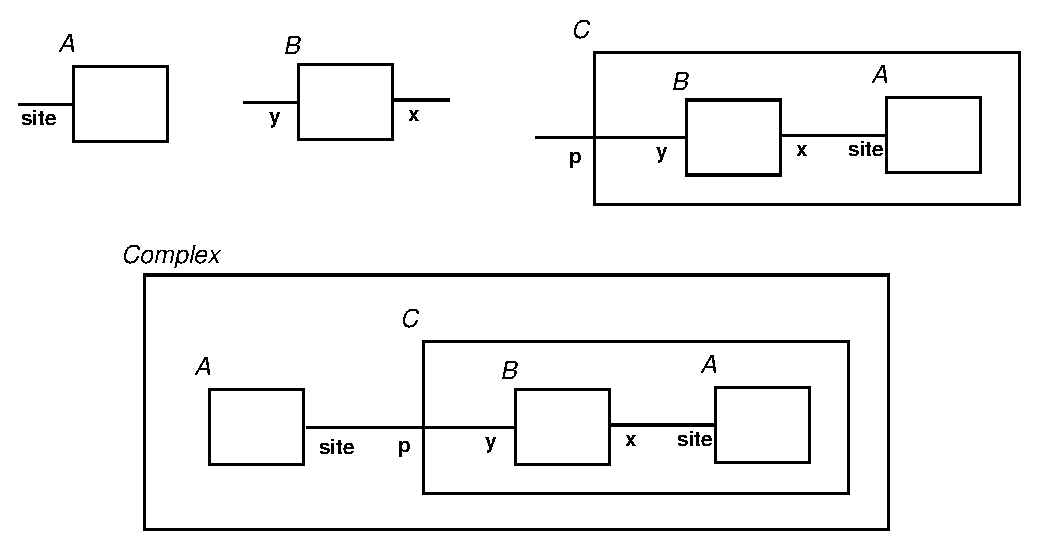
\includegraphics[scale = 0.7]{hierarchial.eps}
\caption{The \texttt{Hierarchical} model which demonstrates the graph encapsulation facilities of
the proposal.  The \texttt{BindingSite} \texttt{p} on \texttt{SpeciesType} \texttt{C} exposes the
uncommitted \texttt{BindingSite} \texttt{y} on \texttt{SpeciesTypeInstance} \texttt{iB}.} 
\label{fig:hierarchial}
\end{figure}

This proposal contains a simple scheme for species type equivalence (described in more detail in
Section~\ref{sec:type-equals}).
This equivalence is used for resolving whether for example the products of different reactions refer
to the same species.
In this scheme
a distinction is made between species types enclosing one or more other species type instances and
those do not.  I'll call those types which do not contain species type instances \emph{simple}
all other types are \emph{complex}.
Simple species types are never equivalent however complex species types can be.  To evaluate the
equivalence of \emph{complex} types we first normalize them into an equivalent form where all species
type instances are \emph{simple} species types.  This normalization process simply removes the
intermediate levels in the hierarchy.  Species type equivalence then considers a normalized 
type as a graph formed by the species type instances, which are graph nodes, and bonds, which are
graph arcs.  
Two species types are equivalent if their graphs are equivalent.
The identity of species types instances normalized complex species types are not relevant
for the purposes of comparing these graphs.
The binding sites of normalized complex species types are also not relevant.

The \texttt{Complex2} \class{SpeciesType} in Figure~\ref{fig:complex2} on Page~\pageref{fig:complex2} is
equivalent to the \texttt{Complex} \class{SpeciesType} in Figure~\ref{fig:hierarchial} on
Page~\pageref{fig:hierarchial}.

\begin{figure}

\begin{example}
<speciesType id="Complex2">
    <listOfSpeciesTypeInstances>
        <speciesTypeInstance id="iA1" speciesType="A"/>
        <speciesTypeInstance id="iA2" speciesType="A"/>
        <speciesTypeInstance id="iB" speciesType="C"/>
    </listOfSpeciesTypeInstances>
    <listOfBonds>
        <specificBond>
            <bindingSiteReference speciesTypeInstance="iA1" bindingSite="site"/>
            <otherBindingSiteReference speciesTypeInstance="iB" bindingSite="y"/>
        </specificBond>
        <specificBond>
            <bindingSiteReference speciesTypeInstance="iA2" bindingSite="site"/>
            <otherBindingSiteReference speciesTypeInstance="iB" bindingSite="x"/>
        </specificBond>
    </listOfBonds>
</speciesType>
\end{example}
  \vspace*{8pt}
  \centering
  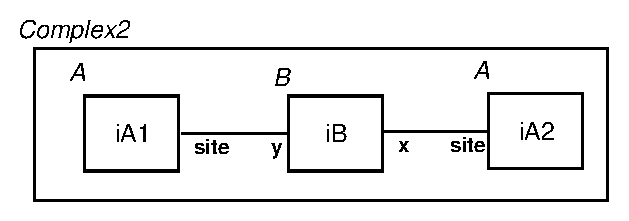
\includegraphics[scale = 0.7]{complex2.eps}
\caption{The \texttt{Complex2} \class{SpeciesType} that is equivalent to the \texttt{Complex} type in
Figure~\ref{fig:hierarchial} on Page~\pageref{fig:hierarchial}} 
\label{fig:complex2}
\end{figure}

\clearpage

\section{Formal Definition of Proposal}
\label{sec:definitions}

\subsection{Proposed Classes in Detail}
This section describes in detail each class in the proposal as shown in
figure~\ref{fig:multi-component-species-uml}.
As in the diagram only new or extended classes are described in this section.
All level 2 structures and basic semantics are assumed to be part of the proposal.
For each new or extended class the definition of the class and its fields are described.

\attrib{id} fields on structures, described here, enclosed within a \class{SpeciesType} structure
are unique to that structure only.
\attrib{id} fields on structures, described here, enclosed within a \class{Reaction} structure are
unique to that reaction only (apart from the \attrib{id} fields of \class{SimpleSpeciesReferences}
which are unique to a whole model).

The definition of \class{species} and \class{speciesType} may not be as one would
expect in conventional biochemical terminology because \class{species} retains its definition
from SBML Level 1 and 2.

\subsubsection{Bond}

The abstract base class \class{Bond} represents one or more chemical bonds or forces holding two chemical
entities together enabling them to form a larger chemical entity.  A \class{bond} can represent
covalent and non-covalent bonds.  The existence of a \class{bond} can imply some
modification of the chemical entities.  For example a phosphorylated protein can be represented
in a model as a \class{bond} between a protein and a phosphate group.  In such a model
the loss of the hydrogen atom bound to the phosphorylation site may or may not be represented
explicitly and does not affect the identity of the protein.  

A \class{Bond} structure consists of one \class{BindingSiteReference} field,
\attrib{bindingSite}, which indicates where the bond has effect.

The linkage of chemical entities together to form a larger chemical entity can be 
represented without using \class{bonds}.  See section~\ref{sec:multicomponentspecies}.

\subsubsection{BindingSite}

A logical site where a bond may form on the chemical entity represented by the
enclosing \class{SpeciesType} structure.  A \class{BindingSite} may represent a set of
physical binding sites which are treated as a single entity for the purposes of the model.  
A \class{BindingSite} structure consists of

\begin{itemize}

\item \attrib{id}, a mandatory \class{SId} field to identify the site

\item \attrib{name}, an optional string field (see SBML Level 2)

\item \attrib{bindingSiteReference}, an optional field containing a
\class{BindingSiteReference} structure.  When this attribute is present the binding site is
exposing an internal binding site on a \class{SpeciesTypeInstance}.
\attrib{bindingSiteReference} refers to a binding site internal to the enclosing
\class{SpeciesType} which is not referenced by another \attrib{bindSiteReference}.

\end{itemize}

A \attrib{bindingSiteReference} value must be present if the enclosing \class{SpeciesType}
contains one or more \attrib{SpeciesTypeInstance} structures.  This means that a
\class{SpeciesType} cannot 'introduce' a new binding site that doesn't exist on
the chemical entites that make up the \class{SpeciesType}.  This restriction is designed to
ensure that evaluating type equivalence is straightforward.

\subsubsection{BindingSiteReference}

A reference to an instance of a \class{BindingSite} in a given \class{SpeciesGraph}.
A \class{BindingSiteReference} structure consists of

\begin{itemize}

\item \attrib{speciesTypeInstance}, a \class{SId} field,
which refers to a \class{SpeciesTypeInstance} within the enclosing
\class{SpeciesGraph}; and

\item \attrib{bindingSite}, a \class{SId} field, which refers to a \class{binding site}
on that instance.  The \class{bindingSite} must be declared on the \class{SpeciesType} referenced by the
\class{SpeciesTypeInstance}).

\end{itemize}

The combination of attribute values of a given \class{BindingSiteReference} structure cannot
occur in any other \class{BindingSiteReference} structure within the same \class{SpeciesGraph}
structure.  

\subsubsection{GenericBond}

Represents a chemical bond between a specific binding site and an unspecified chemical entity which is
unchanged by the reaction.
\class{GenericBond} is a subtype of \class{Bond} and in turn \class{Sbase}.

On \class{GenericBond} the \attrib{id} field, inherited from \class{SBase}, becomes mandatory and
identifies a connection to the unspecified chemical entity.
The \attrib{bindingSiteReference} field represents the binding site that the entity
is connected to.
\class{GenericBond} structures can only occur within \class{Reactions}.
(Specifically they can only occur
in the \class{bond} array/list field in \class{SimpleSpeciesReference}.)
The values of \class{GenericBond} \attrib{id} fields are specific to one reaction. 
All \class{GenericBond} \attrib{id}
fields with the same value in the same reaction refer to the same chemical entity.
\class{GenericBond} \attrib{id} fields in different reactions refer to different chemical entities.

\subsubsection{Model}

See SBML Level 2 for the existing definition of \class{model}.  This proposal adds a
\attrib{speciesType} field which consists of a list of \class{SpeciesType} structures to
\class{Model} structures.  

This proposal changes the definition of the \attrib{species} list on \class{model}.
This list does not necessarily comprise the complete set of pools of chemical entities in the model.
The set of \class{Species} structures in this list which have an undefined or non-zero
initial amount or concentration, \emph{initial species}, are used to infer the complete set
of pools of chemical entities in the model.  The complete set of species located in a given
compartment can be inferred by traversing the reaction
network, defined by the set of \class{Reaction}, from the initial species that are located in
the compartment.

\subsubsection{Reaction}

A reaction
is either located inside a specific compartment, across more than 2 or more compartments or
 potentially in all compartments.  This final case is indicated by the absence of 
\attrib{compartment} and \attrib{species} fields on all enclosed \class{SimpleSpeciesReference}
structures. In this case the \class{SimpleSpeciesReference} structures match with \class{Species}
in the same \class{Compartment} across all compartments in the model.
See section~\ref{sec:commonreaction}

A \class{SpeciesTypeInstance} \attrib{id} field assignment cannot appear more than once within the set of
reactant \class{SpeciesReference} structures on a given reaction.
A \class{SpeciesTypeInstance} \attrib{id} field assignment cannot appear more than once within the set of
product \class{SpeciesReference} structures on a given reaction.

A \class{BindingSiteReference} \attrib{bindingSite} field assignment must appear in both
of reactant and product \class{SpeciesReference} sets on a given reaction.  This means that a 
binding site state determined in the reactants can not be 'lost' from the set of products.

\subsubsection{SimpleSpeciesReference}

See SBML Level 2 for the existing definition of \class{SimpleSpeciesReference}.
\class{SimpleSpeciesReference} is the base class for: (a) \class{SpeciesReference} the type used
to represent the reactants and products of a reaction and (b) \class{ModifierSpeciesReference} the
type used to represent the modifiers of a reaction.  \class{SimpleSpeciesReference} structures
can only occur within a reaction.

In this proposal a \class{SimpleSpeciesReference} can refer to a set of \class{Species} both
those that are explicitly defined and those that are created through generalized reactions
(see section~\ref{sec:generalizedreactions}).  (A \class{SimpleSpeciesReference} on its own does not
imply the existence of a \class{Species}.)

In this proposal a \class{SimpleSpeciesReference} becomes a subtype of \class{SpeciesGraph}.

\class{SimpleSpeciesReference} has the following fields:

\begin{itemize}

\item \attrib{id}, this optional \class{SId} field is not introduced by this proposal but instead
it has a new role: the value of this field can be used as a symbol, enclosed in MathML\texttt{ci}
elements, within the \class{KineticLaw} structure of the enclosing \class{Reaction} structure.

\item \attrib{substanceUnits}, \attrib{spatialSizeUnits} and \attrib{hasOnlySubstanceUnits},
these optional fields have the same semantics as the corresponding attributes on \class{Species}.
These attributes default to the values of matching \class{Species} structures before following the
\class{Species} semnatics.
\class{SimpleSpeciesReference} structures that match with a \class{Species} structure should
default to the \class{Species} attributes and/or be exactly equivalent to them.  Two 
\class{SimpleSpecisReference} structures that refer to the same inferred species should have
the same units.

\item \attrib{species}, this \class{SId} field is present in Level 2 however we now make this field
optional.  This field refers to a \class{Species} that is involved in the reaction.  If this field is
present then the fields inherited from \class{SpeciesGraph} as well as the \attrib{compartment},
\attrib{bond} and \attrib{speciesType} fields are not available.

\item \class{speciesType}, this \class{SId} field refers to a \class{SpeciesType} that is
involved in the reaction.  If this field is
present then the fields inherited from \class{SpeciesGraph} as well as the 
\attrib{Species} and \attrib{bond} fields are not available.  If the \class{compartment}
field is present then the \class{SimpleSpeciesReference} refers to the \class{Species} of
the given \class{SpeciesType} located in the given \class{compartment}; otherwise the
\class{SimpleSpeciesReference} refers to a set of \class{Species} of the given \class{SpeciesType}.

\item \class{compartment}, this \class{SId} field refers to a \class{Compartment} where the matching
\class{Species} are located.  If this field is not present a given \class{SimpleSpeciesReference}
structure then it must not be present on any other 
\class{SimpleSpeciesReference} structure in the same enclosing \class{reaction}.

\end{itemize}

\emph{We might want to consider restricting stoichiometry if \class{SpeciesTypeInstance} structures\
are used.}

\subsubsection{Species}
\label{sec:species}

See SBML Level 2 for the existing definition of \class{Species}.  In this proposal a 
\class{Species} structure represents a pool of a given chemical entity located in a specific
compartment. 
This proposal introduces one optional \class{SId} field, \attrib{speciesType} which refers to
the \class{SpeciesType} (chemical entity) to be located in the \class{Compartment} referenced by
the \attrib{compartment} field.  There can only one \class{Species} structure in a model with a given
pair of values for the \attrib{speciesType} and \attrib{compartment} attributes i.e.
a given \class{SpeciesType} cannot be located in the same \attrib{Compartment} mode than once.

\emph{revise this:}
When the \attrib{speciesType} field is not present then the \class{Species} structure is equivalent
to a \class{Species} structure which does contain a \attrib{speciesType} field.
This field would refer to a \class{SpeciesType} that is not referenced anywhere else in the model.
In short a \class{Species} structure without a \attrib{speciesType} field has a
`hidden' \class{SpeciesType} associated with it.

\subsubsection{SpeciesGraph}

\class{SpeciesGraph} is an abstract base class.
A \class{SpeciesGraph} structure represents a chemical entity or a set of chemical entities of
a specific common form.  The form of these entities is defined as a graph where the nodes are
\class{SpeciesTypeInstances} and the arcs are \class{Bond} structures.  The graph can be disconnected
indicating that the detail of how parts of the chemical entities are associated are not relevant to the
model (see~\ref{sec:multicomponentspecies}).  

A \class{SpeciesGraph} structure is composed of the following fields:

\begin{itemize}

\item \attrib{speciesTypeInstance}, this is an optional list of \class{SpeciesTypeInstance}
structures that form the \class{SpeciesGraph}.  If this list is not present
then the \class{SpeciesGraph} simply represents an chemical entity for which the detail
of its composition is not relevant to the model.

\item \attrib{unboundSite}, this is an optional list of \class{BindingSiteReference} structures which
refer to the binding sites on the \class{SpeciesTypeInstance} structures in the \class{SpeciesGraph}
which are unbound (not part of a \class{Bond}).  In model an unbound binding site may have
some implied chemical structure which is not made explicit i.e. the binding site may not be physically
unoccupied and the entity occupying the site is simply not modelled.

\item \class{bond}, an optional list of \class{Bond} structures that can include both
\class{SpecificBond} and \class{GenericBond} structures.
This list links the chemical entities 
enumerated in the \attrib{speciesTypeInstance} field.

\end{itemize}

\subsubsection{SpeciesType}

The class \class{SpeciesType} represents a specific
chemical entity.  \class{SpeciesType} is derived from \class{SpeciesGraph}, and has the following fields:

\begin{itemize}

\item \attrib{id} a mandatary \class{SId} field that identifies the \class{SpeciesType}

\item \attrib{name}, an optional string field (see SBML Level 2)

\item \attrib{bindingSite}, an optional \class{BindingSite} list, which contains the set of binding
sites that are located on the \class{SpeciesType}.

\end{itemize} 

A simple example of the use \class{SpeciesType} structures is given in section~\ref{sec:commonspecies}.

Consider all the \class{BindingSite} structures of the \class{SpeciesType}
structures referenced by the species type instances in a given \class{SpeciesType}
structure.  Each of these \class{BindingSite} structures should be referenced exactly once by a
\class{Bond} structure enclosed in the \class{SpeciesType} structure.  This means that
the status of a \class{BindingSite} can't be left undefined or ambiguous by a \class{SpeciesType}.

\subsubsection{SpeciesTypeInstance}

A \class{SpeciesTypeInstance} structure represents the occurrence of a chemical entity of a given
\class{SpeciesType} within a \class{SpeciesGraph}.  A \class{SpeciesTypeInstance} structure has the
following fields:

\begin{itemize}

\item \attrib{id} a mandatory \class{SId} field that identifies the \class{SpeciesTypeInstance}.
This field is unique to the enclosing \class{SpeciesGraph} structure and the enclosing
\class{Reaction} structure if it exists.

\item \attrib{name}, an optional string field (see SBML Level 2)

\item \attrib{speciesType}, a mandatory \class{SId} field which refers to the \class{SpeciesType}
that the \class{SpeciesTypeInstance} is an instance of.

\end{itemize}

\subsubsection{SpecificBond}

A subtype of \class{Bond}.   \class{SpecificBond} represents either (a) one or more chemical bonds
between two explicitly identified binding sites or (b) an unoccupied binding site.  A \class{bond}
structure consists of two
structures
\attrib{bindingSite} and
\attrib{otherBindingSiteReference} which are \class{bindingSiteReference} structures.

\attrib{bindingSite} is inherited from \class{Bond}.
\attrib{otherBindingSiteReference} is optional.
The \class{SpecificBond} structure represents the state in which \attrib{bindingSite} is unbound if
\attrib{otherBindingSiteReference} is not present.
If \attrib{otherBindingSiteReference} is present the \attrib{bindingSite} and
\attrib{otherBindingSiteReference} fields represent the 2 binding sites that are linked by a bond.
Neither binding site has privileged semantics.
See section~\ref{sec:explicitbonds} for examples.

\subsection{Equivalence of Species Types}

\label{sec:type-equals}

This section defines the equivalence of \class{SpeciesType} structures.
This is defined as a process with 3 stages described by the following 
sections in order.  First the \class{SpeciesType} structures are transformed into a
standard \emph{complex} form of \class{SpeciesGraph}, as described in Section~\ref{sec:trans-type}.
Second these \class{SpeciesGraph}
are normalized (flattened), as described in Section~\ref{sec:norm-graphs}.
Finally if these normalized structures can the be
matched, as decribed in Section~\ref{sec:match-graphs},
then the \class{SpeciesType} structures are equivalent. 

\subsubsection{Normalization of Species Types}
\label{sec:trans-type}

This section describes how a \class{SpeciesType} is normalized.

A \class{SpeciesGraph} is \emph{simple} if it contains no \class{SpeciesTypeInstance} structures.
A \class{SpeciesGraph} is \emph{complex} if it contains one or more \class{SpeciesTypeInstance} structures.

A normalized \class{SpeciesType} is always complex.
A simple \class{SpeciesType} structure is normalized by creating a \class{SpeciesGraph}
that contains one \class{SpeciesTypeInstance} structure which refers to the simple \class{SpeciesType}.
All binding sites of the simple \class{SpeciesType} are referenced as unbound in a set of
\class{SpecificBonds} within the new normalized \class{SpeciesGraph}.

A complex \class{SpeciesType} with one or more \class{BindingSite} structures is transformed
to remove the those structures.  Each \class{BindingSite} structure is replaced by a
\class{SpecificBond} structure containing just the \class{BindingSiteReference} structure
that was contained in the \class{BindingSite} structure.  This means that the original
binding sites are made unbound by the normalization process
(instead of being avaliable for binding in a different context).

Once the rules have been applied the \class{SpeciesType} is normalized as described in
Section~\ref{sec:norm-graphs}.

\subsubsection{Normalization of Species Graphs}
\label{sec:norm-graphs}

This section describes how the form of species graphs is normalized for 
the matching process.  This normalization process simply reduces the
given Species Graph to a single hierarchical level.

A \class{SpeciesGraph} structure (i.e. either a \class{SpeciesType} or \class{SimpleSpecies}
structure) is normalized if the set of \class{SpeciesType} structures, refereed to by the set
of \class{SpeciesTypeInstance} structures, are simple.  
The normalization process consists of iteratively replacing any \class{SpeciesTypeInstance} structures
that refer to complex \class{SpeciesType} structures with a set of new
\class{SpeciesTypeInstance} structures and \class{SpecificBond} structures that are copies of that
occurring within the complex \class{SpeciesType} structure.  These new structures are linked into
the same 'outer' \class{Bond} structures as the initial complex \class{SpeciesType} structure.

\subsubsection{Normalized Species Graph Equivalence}
\label{sec:match-graphs}

When evaluating the equivalence of \class{SpeciesGraph} structures the following aspects
are not directly relevant:
\begin{itemize}
\item \class{id} on \class{SpeciesTypeInstance}
\item the order of structures within lists
\class{SpecificBond} structures representing unbound binding sites
\end{itemize}

The \class{id} on \class{SpeciesTypeInstance} is only used to provide linkage within a single
graph.

In this section we consider a normalized \class{SpeciesGraph} to be a formal graph and
equivalence to be a graph matching operation.  A formal representation of graph is

\textbf{Definition} (A Simple Graph) A \emph{simple graph} $G$ is a
tuple $G = (G_{V}, G_{E}, L, I, J, s, t, \ell, i, j)$
consisting of
\begin{itemize}

\item a finite set of nodes (or ``vertices'') $G_{V}$ and a finite set of arcs (or ``edges'') $G_{E}$
        where $G_{v} \cap G_{E} = \emptyset$,

\item two total mappings $s, t : G_{E} \rightarrow G_{V}$ (``source and target''),

\item a set of node labels $L$,

\item a set of arc source labels $I$,

\item a set of arc target labels $J$,

\item a total mapping $\ell : G_{V} \rightarrow L$ (``node labelling'')

\item a total mapping $i : G_{E} \rightarrow I$ (``arc source labelling'')

\item a total mapping $j : G_{E} \rightarrow J$ (``arc target labelling'')

\end{itemize}
The nodes and arcs of a graph are also collectively called the ``objects'' of the graph
(or ``graph objects'').  Note that in this definition that we are labelling the source and 
target 'ends' of each arc.

\emph{ modified from \citep{rudolf:1998}}

In this formulation of the formal graphs
the graph nodes, $G_{V}$, are the \class{SpeciesTypeInstance} structures and
the arcs, $G_{E}$, are the \class{SpecificBond}
structures.  The source and target of an arc is determined by the \attrib{speciesTypeInstance} field
of the \class{BindingSiteReference} structures enclosed in the given \class{SpeciesBond}.
The arc direction (the distinction between the source and target) is determined by a consistent ordering
over \attrib{speciesType} attributes of the \attrib{speciesTypeInstance} structures.  

The label, $\ell(v)$ of a node, $v$ is its
\attrib{speciesType} attribute.  The arc source label, $i(e)$ of an arc, $e$, is formed from the
\attrib{bindingSite} attribute of the given source \class{BindingSiteReference} structure.
The arc target label, $j(e)$ of an arc, $e$, is formed from the
\attrib{bindingSite} attribute of the given target \class{BindingSiteReference} structure.

Two \class{SpeciesGraph} structures are equivalent if their normalized forms as 
graphs match in both directions.  Formally a match of one graph into another is given by a
graph morphism, which is a mapping of one graph's object
sets into the other's, with some restrictions to preserve the graph's structure and it's typing
information:

\textbf{Definition} (Graph Morphism) A \emph{graph morphism} $m : L \rightarrow G$ between two
simple graphs
\begin{itemize}
\item $L = (L_{V}, L_{E}, L_{L}, I_{L}, J_{L}, s_{L}, t_{L}, \ell_{L}, i_{L}, j_{L})$ and
\item $G = (G_{V}, G_{E}, L_{G}, I_{G}, J_{G}, s_{G}, t_{G}, \ell_{G}, i_{G}, j_{G})$
\end{itemize}
is a pair of total mappings
$m = (m_{V} : L_{V} \rightarrow G_{V}, m_{E} : L_{E} \rightarrow G_{E})$,
where the following restrictions apply:

\begin{enumerate}
\item $\forall e \in L_{E} : $
    \begin{itemize}
    \item $m_{V}(s_{L}(e))= s_{G}(m_{E}(e))$
    \item $m_{V}(t_{L}(e))= t_{G}(m_{E}(e))$
    \end{itemize}
\item $\forall v \in L_{V} : \ell_{L}(v) = \ell_{G}(m_{V}(v))$
\item $\forall e \in L_{E} : i_{L}(e) = i_{G}(m_{E}(e))$
\item $\forall e \in L_{E} : j_{L}(e) = j_{G}(m_{E}(e))$
\end{enumerate}

\emph{modified from \citep{rudolf:1998}}

\subsubsection{Implications of \class{SpeciesType} Equivalence}

Two or more equivalent \class{SpeciesType} structures can co-exist in the same model
(the \attrib{id} attributes must have different values).  Section~\ref{sec:species-equals}
describes how \class{Species} equivalence is derived from \class{SpeciesType} equivalence.

\subsection{\class{Species} Equivalence}
\label{sec:species-equals}

Two \class{Species} are equivalent if they are located in the same compartment and their associated
\class{SpeciesType} structures are equivalent.  A model must not contain equivalent \class{Species}.
The species implied by the reactions in a model, described in Section~\ref{sec:reaction-semantics},
are inherently not equivalent.

\subsection{Semantics of Reactions}
\label{sec:reaction-semantics}
\subsubsection{Simple Framework for Operational Semantics}

For the definition of the semantics of reactions we will consider a model with a simulator to be form of
AI \emph{production system}.

\begin{quote}
The major elements of an AI production system are a \emph{global database}, a set of
\emph{production rules}, and a \emph{control system}.
[...]
Depending on the application, this database may be as simple as a small matrix of numbers or as
complex as a large, relational, index file structure.  (The reader should not confuse the phrase,
``global database,'' as it is used [here], with the databases of database systems.)

The production rules operate on the global database.  Each rule has a \emph{precondition} that is either
satisfied or not by the global database.  If the precondition is satisfied, the rule can be
\emph{applied}.  Application of the rule changes the database.  The control system chooses which
applicable rule should be applied and ceases computation when a termination condition on the global
database is satisfied.~\citep{Nilsson:1982}
\end{quote}

In the context of this proposal reactions are considered to be rules.  
The global database is formed by
the modelled species which are pools of chemical entities.  
In SBML Level 2 the set of \class{Species} structures defines the complete set of pools of chemical
entities that are created by, destroyed by and affect the set of reactions. In this proposal the set of
\class{Species}
structures only describes the initial conditions of the model.  The reactions themselves define the
species or set of pools of entities that are relevant to the model. 
It is expected that any analysis of a model will require the computation of the set of species.
This proposal does not depend on any particular representation scheme for species within a given
software analysis system.

A reaction matches
the set of reactants, its precondition, to the set of species, the global database.  The effect of the
reaction is to remove reactant entities and create product entities within the set of species.
The existence of a modifier entity is not a pre-condition of a reaction however the number of
chemical entities in the modifier's pool will affect the reaction according to the reaction's
rate law.

For the purposes of this definition the control system is idealized. Real software systems will in
practice create approximations of this control system.  The ideal control system simply applies all
matching reactions concurrently at the rate defined by the reaction' kinetic laws.  Unlike a AI
production system this proposal does not define any termination conditions.  

\subsubsection{Matching of Species}

This section describes how reactions are matched to the global database of species.

\emph{Unification of Species to Reactants and Modifiers}

The matching of reactant and modifiers, \class{SimpleSpeciesReference} structures,
to species is similar to equivalence between species.  
The cases we will consider with respect to the \class{SimpleSpeciesReference} are:
\begin{itemize}

\item \emph{\attrib{species} attribute is present}, in this case the match is with the indicated
\class{Species}.

\item \emph{\attrib{speciesType} and \attrib{compartment} attributes are present}, in this case the match is
with the species located in the given \class{Compartment} which has a \class{SpeciesType} equivalent to
the given \class{SpeciesType}.

\item \emph{\attrib{speciesType} is present but the \attrib{compartment} attribute is not present},
in this case the match is
with any species which has a \class{SpeciesType} equivalent to
the given \class{SpeciesType}.  The \class{Compartment} of the species must be the same as
all other species involved in the reaction.

\item \emph{all of the remaining cases} are described below.
\end{itemize}

In the remaining cases the matching between \class{SimpleSpeciesReference} and species
is considered to be a variant of \class{SpeciesType} equivalence.  If the \attrib{compartment}
attribute is not present on the \class{SimpleSpeciesReference} then the match is with any
species matching the \class{SpeciesType} located in the same \class{Compartment} as all the other
species involved in the reaction.  If the \attrib{compartment} attribute is present then
the match is with any species matching the \class{SpeciesType} located in the given \class{Compartment}.

To enable the definition of a match between a \class{SimpleSpeciesReference} and a \class{SpeciesType}
we first require a definition of a \emph{generic graph} and definition of \class{SimpleSpeciesReference}
in terms of a \emph{generic graph}.  (The use \emph{generic graph} here is to capture the semantics of 
\class{GenericBond} structures which may be contained within a \class{SimpleSpeciesReference}.)

\textbf{Definition} (A Generic Graph) A \emph{generic graph} $G$ is a tuple
$G = (G_{V}, G_{E}, G_{X}, L, I, J, s, t, u, \ell, i, j)$
consisting of
\begin{itemize}

\item a finite set of nodes (or ``vertices'') $G_{V}$, a finite set of arcs (or ``edges'') $G_{E}$
and a finite set of generic nodes $G_{X}$ where
    \begin{enumerate}
    \item $G_{V} \cap G_{E} = \emptyset$
    \item $G_{V} \cap G_{X} = \emptyset$
    \item $G_{E} \cap G_{X} = \emptyset$
    \end{enumerate}
    
\item two total mappings $s, t : G_{E} \rightarrow G_{V}$ (``source and target''),

\item a total mapping $u : G_{X} \rightarrow G_{V}$ (``generic connection''),

\item a set of arc source labels $I$,

\item a set of arc target labels $J$,

\item a total mapping $\ell : G_{V} \cup G_{X} \rightarrow L$ (``node labelling'')

\item a total mapping $i : G_{E} \rightarrow I$ (``arc source labelling'')

\item a total mapping $j : G_{E} \rightarrow J$ (``arc target labelling'')

\end{itemize}
The nodes, generic nodes and arcs of a graph are also collectively called the ``objects'' of the
generic graph (or ``generic graph objects'').

The formulation of a \class{SimpleSpeciesReference} as a generic graph similar to that
of a \class{SpeciesType} to a simple graph.
The graph nodes, $G_{V}$, are the \class{SpeciesTypeInstance} structures,
arcs, $G_{E}$, are the \class{SpecificBond} structures and generic nodes, $G_{X}$, are the
\class{GenericBond} structures.  The source, $s$ and target, $t$, of an arc are determined by the
\attrib{speciesTypeInstance} field of the \class{BindingSiteReference} structures enclosed in the given
\class{SpeciesBond}.  The arcs are directed
where arc direction should be determined using an consistent ordering over the set of simple species
types.
The generic connections of a generic node, $u$ are determined by the \attrib{speciesTypeInstance} field
of the \class{BindingSiteReference} structure enclosed in the given \class{GenericBond}. 
For our purposes the label or type of a node is its
\attrib{speciesType} attribute and the label or type of an arc is formed from the pair of
\attrib{bindingSite} attributes of the given \class{SpecificBond} structures.
The arc direction determines the ordering of each arc's \attrib{bindingSite}
attributes in the arc's label.
The label of generic node is the \attrib{bindingSite} attribute of the given
\class{GenericBond} structure.

A match of generic graph (from a \class{SimpleSpeciesReference}) into a simple graph
(from a \class{SpeciesType} as described in Section~\ref{sec:match-graphs}) is given by a graph
morphism, which is a mapping of the generic graph's object
sets into the simple graph's, with some restrictions to preserve the generic graph's structure and
it's typing information:

\textbf{Definition} (Generic Graph Morphism) A \emph{generic graph morphism}
$m : L \rightarrow G$ between
\begin{itemize}
\item a generic graph
$L = (L_{V}, L_{E}, L_{X}, L_{L}, I_{L}, J_{L}, s_{L}, t_{L}, u_{L}, \ell_{L}, i_{L}, j_{L})$ and
\item a simple graph $G = (G_{V}, G_{E}, L_{G}, I_{G}, J_{G}, s_{G}, t_{G}, \ell_{G}, i_{G}, j_{G})$
\end{itemize}
is a pair of total mappings
$m = (m_{V} : L_{V} \rightarrow G_{V}, m_{E} : L_{E} \cup L_{X} \rightarrow G_{E})$
where the following restrictions apply:

\begin{enumerate}
\item $\forall x \in L_{X} : m_{V}(u(x)) = s_{G}(m_{E}(x)) \vee m_{V}(u(x)) = t_{G}(m_{E}(x))$
\item $\forall e \in L_{E} : $
    \begin{itemize}
    \item $m_{V}(s_{L}(e))= s_{G}(m_{E}(e))$
    \item $m_{V}(t_{L}(e))= t_{G}(m_{E}(e))$
    \end{itemize}
\item $\forall v \in L_{V} : \ell_{L}(v) = \ell_{G}(m_{V}(v))$
\item $\forall e \in L_{E} : i_{L}(e) = i_{G}(m_{E}(e))$
\item $\forall e \in L_{E} : j_{L}(e) = j_{G}(m_{E}(e))$
\item $ \forall x \in L_{X} : \ell_{L}(x) = \left\{
\begin{array}{ll}
i_{G}(m_{E}(x)) & \mbox{if $m_{V}(u(x)) = s_{G}(m_{E}(x))$}\\
j_{G}(m_{E}(x)) & \mbox{if $m_{V}(u(x)) = t_{G}(m_{E}(x))$}
\end{array} \right. $
\end{enumerate}

The mapping $m_{E}$ from the set of generic bonds, $L_{X}$ to specific bonds, $G_{E}$ 
represents a set of assignments which are used to determine the effect of a reaction.
This is described further in Section~\ref{sec:effect-of-reactions}. 

\subsubsection{Matching Reactions}

A \class{Reaction} which does not contain any \class{GenericBond} structures represents a single
\emph{reaction instance}.  A \class{Reaction} that does contain \class{GenericBond} structures
represents a set of reaction instances where each instance in this set is a concrete reaction
with generic graph mappings for all the reactant and modifier \class{SimpleSpeciesReference} structures.
There is a separate reaction instance for all possible combinations of these graph mappings.
Each reaction instance exists concurrently with the other instance and operates at the
rate determined by the reaction's kinetic law.

\emph{This means that some care must be taken when formulating the kinetic laws of reactions containing
\class{GenericBond} structures.  Typically to obtain the correct results kinetic laws should be defined
so that the rate of the reaction is directly proportional to the amount of the species matched
using \class{GenericBond} structures.}

\subsubsection{The Effect of Reactions}
\label{sec:effect-of-reactions}

A reaction reduces the amount of the reactant species and increases the amount of the product
species.  A reaction does not affect the amount of a Modifier species (unless its a reactant or product).
If the species graph for a product which doesn't contain \class{GenericBond} structures it can be
matched to a species as for reactants.

In a reaction instance any product \class{GenericBond} structures are eliminated by viewing the effect of
a reaction as graph transformation process.
The resulting \emph{concrete} product can then be matched to species.
In this transformation process we take each set of matching reactant species graphs 

\subsubsection{Reversible reactions}

%\clearpage
%\section{Discussion}
%
%\subsection{Modifiers and species inference}
%
%\subsection{Use of generic bonds in \class{SpeciesType} structures}
%
%\subsection{Connections between Generic Bonds}
%
%\subsection{Option - Reaction Predicates}
%
%\subsection{Option - SpeciesType inheritance}
%
%\subsection{Discussion - Model Composition and Multi-component Species}
%
%\subsection{Discussion - reaction specificity - do we need groups?}
%
%\subsection{Discussion - Attributes of Species and Species Types}

\newpage
\section{Appendix}
\setcounter{secnumdepth}{2}
\appendix

\section{Elements introduced in this proposal}
\section{Attributes introduced in this proposal}
%=============================================================================
% References
%=============================================================================

\bibliographystyle{apalike}
\bibliography{strings,a,b,c,d,e,f,g,h,i,j,k,l,m,n,o,p,q,r,s,t,u,v,w,x,y,z}
\end{document}
